\setchaptergraphic{
    % Dodecahedron
    \begin{tikzpicture}[scale=1.5,line join=bevel,z=-5.5]
        \tikzmath{\goldenratio = 0.5*(1 + sqrt(5));}

        \coordinate (A1) at (1,1,1);
        \coordinate (A2) at (1,1,-1);
        \coordinate (A3) at (1,-1,1);
        \coordinate (A4) at (1,-1,-1);
        \coordinate (A5) at (-1,1,1);
        \coordinate (A6) at (-1,1,-1);
        \coordinate (A7) at (-1,-1,1);
        \coordinate (A8) at (-1,-1,-1);

        \coordinate (B1) at (0,\goldenratio,1/\goldenratio);
        \coordinate (B2) at (0,\goldenratio,-1/\goldenratio);
        \coordinate (B3) at (0,-\goldenratio,1/\goldenratio);
        \coordinate (B4) at (0,-\goldenratio,-1/\goldenratio);

        \coordinate (C1) at (1/\goldenratio, 0, \goldenratio);
        \coordinate (C2) at (-1/\goldenratio, 0, \goldenratio);
        \coordinate (C3) at (1/\goldenratio, 0, -\goldenratio);
        \coordinate (C4) at (-1/\goldenratio, 0, -\goldenratio);

        \coordinate (D1) at (\goldenratio, 1/\goldenratio, 0);
        \coordinate (D2) at (\goldenratio, -1/\goldenratio, 0);
        \coordinate (D3) at (-\goldenratio, 1/\goldenratio, 0);
        \coordinate (D4) at (-\goldenratio, -1/\goldenratio, 0);

        \draw[black] (B1) -- (B2);
        \draw[black,dashed] (B3) -- (B4);

        \draw[black] (C1) -- (C2);
        \draw[black, dashed] (C3) -- (C4);

        \draw[black] (D1) -- (D2);
        \draw[black] (D3) -- (D4);

        \draw[black] (A1) -- (B1);
        \draw[black] (A1) -- (C1);
        \draw[black] (A1) -- (D1);

        \draw[black] (A2) -- (B2);
        \draw[black, dashed] (A2) -- (C3);
        \draw[black] (A2) -- (D1);

        \draw[black] (A3) -- (B3);
        \draw[black] (A3) -- (C1);
        \draw[black] (A3) -- (D2);

        \draw[black, dashed] (A4) -- (B4);
        \draw[black, dashed] (A4) -- (C3);
        \draw[black, dashed] (A4) -- (D2);

        \draw[black] (A5) -- (B1);
        \draw[black] (A5) -- (C2);
        \draw[black] (A5) -- (D3);

        \draw[black] (A6) -- (B2);
        \draw[black, dashed] (A6) -- (C4);
        \draw[black] (A6) -- (D3);

        \draw[black] (A7) -- (B3);
        \draw[black] (A7) -- (C2);
        \draw[black] (A7) -- (D4);

        \draw[black, dashed] (A8) -- (B4);
        \draw[black, dashed] (A8) -- (C4);
        \draw[black, dashed] (A8) -- (D4);

        \fill[opacity=0.7,fill=green!50!black] (D4) -- (D3) -- (A5) -- (C2) -- (A7) -- cycle;
        \fill[opacity=0.7,fill=green!50!black] (A6) -- (D3) -- (A5) -- (B1) -- (B2) -- cycle;

        \fill[opacity=0.7,fill=green!30!blue] (B2) -- (B1) -- (A1) -- (D1) -- (A2) -- cycle;
        \fill[opacity=0.7,fill=green!30!blue] (D1) -- (A1) -- (C1) -- (A3) -- (D2) -- cycle;

        \fill[opacity=0.7,fill=orange!50!black] (C1) -- (C2) -- (A7) -- (B3) -- (A3) -- cycle;
        \fill[opacity=0.7,fill=blue!30!red] (C1) -- (C2) -- (A5) -- (B1) -- (A1) -- cycle;
    \end{tikzpicture}
}

\chapter{Group Theory}
\label{ch:groups}

\section{Symmetries}

Our first motivation for studying groups will be the symmetries of regular $n$-gons, starting with the regular $3$-gon: the equilateral triangle. The symmetries of a regular $n$-gon in the plane are rotations and reflections which take the $n$-gon to itself.

For example, if we take an equilateral triangle and label the vertices $A, B, C$, in anti-clockwise order starting from the top, we have two rotational symmetries: rotation by $120^\circ$ and rotation by $240^\circ$, in a particular sense or direction, say anti-clockwise. We also have three reflection symmetries --- reflections across a line going from one vertex to the midpoint of the opposite edge.

\begin{figure}[ht!]
    \centering
    \begin{tikzpicture}
        \coordinate (A1) at (0, {sqrt(3)});
        \coordinate (B1) at (-1, 0);
        \coordinate (C1) at (1, 0);
        \coordinate (R1) at ($(B1)!0.5!(C1)$);
        \coordinate (R11) at ($(A1)!1.25!(R1)$);
        \coordinate (R12) at ($(R1)!1.25!(A1)$);

        \node[anchor=south east] at (A1) {$A$};
        \node[anchor=east] at (B1) {$B$};
        \node[anchor=west] at (C1) {$C$};

        \draw [thick] (A1)--(B1);
        \draw [thick] (B1)--(C1);
        \draw [thick] (C1)--(A1);

        \draw [thick, dashed] (R11)--(R12);

        \coordinate (A2) at (4, {sqrt(3)});
        \coordinate (B2) at (5, 0);
        \coordinate (C2) at (3, 0);
        \coordinate (R2) at ($(B2)!0.5!(C2)$);
        \coordinate (R21) at ($(A2)!1.25!(R2)$);
        \coordinate (R22) at ($(R2)!1.25!(A2)$);

        \node[anchor=south east] at (A2) {$A$};
        \node[anchor=west] at (B2) {$B$};
        \node[anchor=east] at (C2) {$C$};

        \draw [thick] (A2)--(B2);
        \draw [thick] (B2)--(C2);
        \draw [thick] (C2)--(A2);

        \draw [thick, dashed] (R21)--(R22);
    \end{tikzpicture}
\caption{Reflection symmetry $S_1$}
\label{fig:triangle-reflection}
\end{figure}

Let $R$ be the rotation by $120^\circ$ anti-clockwise. Then the rotation by $240^\circ$ anti-clockwise is simply $R$ applied twice, so we will denote it by $R^2$. Let $S_1$ be the reflection symmetry across the line through the top vertex, $S_2$ across the line through the left vertex, and $S_2$ the right vertex. The final symmetry is the identity transform, which we will call $e$. The triangle therefore has six symmetries in total: $\{e, S_1, S_2, R, R^2\}$.

\begin{figure}[ht!]
    \centering
    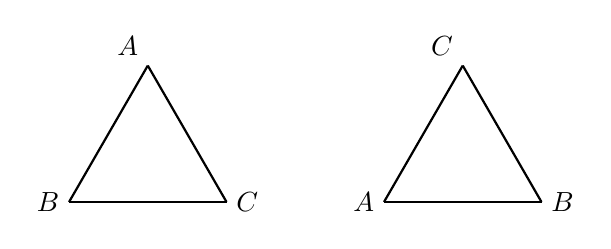
\begin{tikzpicture}
        \coordinate (A1) at (0, {sqrt(3)});
        \coordinate (B1) at (-1, 0);
        \coordinate (C1) at (1, 0);

        \node[anchor=south east] at (A1) {$A$};
        \node[anchor=east] at (B1) {$B$};
        \node[anchor=west] at (C1) {$C$};

        \draw [thick] (A1)--(B1);
        \draw [thick] (B1)--(C1);
        \draw [thick] (C1)--(A1);

        \coordinate (A2) at (3, 0);
        \coordinate (B2) at (5, 0);
        \coordinate (C2) at (4, {sqrt(3)});

        \node[anchor=east] at (A2) {$A$};
        \node[anchor=west] at (B2) {$B$};
        \node[anchor=south east] at (C2) {$C$};

        \draw [thick] (A2)--(B2);
        \draw [thick] (B2)--(C2);
        \draw [thick] (C2)--(A2);
    \end{tikzpicture}
\caption{Rotation symmetry $R$}
\label{fig:triangle-rotation}
\end{figure}

Since every symmetry takes the triangle to itself, products (compositions) of Symmetries are themselves symmetries. If $u$ and $w$ are symmetries, let $uw$ denote the composition of first $w$ and then $u$ after the manner of function composition. For example, $S_1S_2 = R$, $RR = R^2$, and $R^2R = e$.

Note that multiplication of symmetries is not necessarily commutative: $S_1S_2 = R$, but $S_2S_1 = R^2$. Multiplication with the identity is however commutative: $eR^2 = R^2 = R^2e$, etc.

We can construct a full multiplication table for the six symmetries of the $3$-gon listing all possible binary products, which is shown in Table \ref{triangle-multiplication-table}.

\begin{minipage}{\linewidth}
    \begin{center}
    \captionof{table}{Group multiplication table for $3$-gon}
    \label{triangle-multiplication-table}
    \begin{tabular}{|c||c|c|c|c|c|c|}
    \hline
    \thead{$\circ$} & \thead{$e$} & \thead{$S_1$} & \thead{$S_2$} & \thead{$S_3$} & \thead{$R$} & \thead{$R^2$}\\
    \hline\hline
    $e$   & $e$   & $S_1$ & $S_2$ & $S_3$ & $R$   & $R^2$ \\ \hline
    $S_1$ & $S_1$ & $e$   & $R$   & $R^2$ & $S_2$ & $S_3$ \\ \hline
    $S_2$ & $S_2$ & $R^2$ & $e$   & $R$   & $S_3$ & $S_1$ \\ \hline
    $S_3$ & $S_3$ & $R$   & $R^2$ & $e$   & $S_1$ & $S_2$ \\ \hline
    $R$   & $R$   & $S_3$ & $S_1$   & $S_2$ & $R^2$ & $e$   \\ \hline
    $R^2$ & $R^2$ & $S_2$ & $S_3$ & $S_1$ & $e$   & $R$   \\ \hline
    \end{tabular}
    \end{center}
\end{minipage}

\section{Group Axioms}

\begin{defn}
    A \emph{group} $G$ is a set together with a closed binary operation on the elements of the set (typically called ``multiplication'') that satisfies the following axioms:
    \begin{itemize}
        \item There exists an identity element $e \in G$ such that $ex = x = xe$ for every $x \in G$.
        \item Every element $x \in G$ has an inverse $x^{-1}$ such that $xx^{-1} = e$.
        \item The operation is associative: $x(yz) = (xy)z$, for every $x, y, z \in G$.
    \end{itemize}
\end{defn}

\begin{exmp}
    The symmetries of a triangle $\{e, S_1, S_2, S_3, R, R^2\}$, together with the binary operation of composition, form a group. Table \ref{triangle-multiplication-table} shows that every element has an inverse and that composition of these symmetries is closed. Associativity comes from the fact that $(xy)z$ means apply the symmetry $z$, then $y$, and then $x$, and $x(yz)$ also means apply $z$, then $y$, and then $x$, so the result is the same and $(xy)z = x(yz)$.
\end{exmp}

\begin{exmp}
    $\N$, $\Z$, $\Q$, $\R$, and $\C$ all form groups under addition, and $\Q - \{0\}$, $\R - \{0\}$, and $\C - \{0\}$ form groups under multiplication.
\end{exmp}

\begin{exmp}
    $\{1, -1, i, -i\} \subset \C$ forms a group under complex multiplication. It can be easily verified it is closed under multiplication, $1$ is the identity, and it inherits associativity from $\C$. Inverse can be easily checked: $(-1)(-1) = 1$ and $i(-i) = 1$.
\end{exmp}

\begin{defn}
    If a group is commutative, then it is an \emph{abelian} group.
\end{defn}

\begin{defn}
    The \emph{order} of a group is the cardinality of the group.
\end{defn}

\begin{defn}
    A \emph{subgroup} $H$ of a group $G$ is a set $H \subseteq G$ that forms a group under the same group operation as $G$. If $H$ is a subgroup of $G$ this may be denoted by $H \leqslant G$, or $H < G$ if it is a strict subgroup.
\end{defn}

\begin{thm}\label{subgroup-test}
    A non-empty subset $H$ of a group $G$ is a subgroup of $G$ if and only if $x, y \in H$ implies $xy^{-1} \in H$.
\end{thm}

\begin{proof}\proofbreak
    ($\implies$) If $H$ is a subgroup of $G$, then since $y \in H$ it must be that $y^{-1} \in H$. Since groups are closed under the group operation, $x, y^{-1} \in H$ then implies that $xy^{-1} \in H$.

    ($\impliedby$) Since $H$ is non-empty, there must exist some $x \in H$, and so $xx^{-1} \in H$, which implies $H$ contains the identity. $H$ clearly inherits associativity from $G$, so it only remains to check that it contains inverses and is closed. Since $e, x \in H$, $ex^{-1} \in H$, but $ex^{-1} = x^{-1}$ so $H$ contains all inverses. Finally, if $x, y \in H$, we also have $x, y^{-1} \in H$, so $xy \in H$ and so $H$ is closed.
\end{proof}

\begin{thm}
    Let $H, K \subseteq G$ be subgroups. Then $H \intersection K$ is a subgroup of $G$.
\end{thm}

\begin{proof}
    Since $e \in H$ and $e \in K$, we of course have $e \in H \intersection K$. If $x \in H \intersection K$, then $x^{-1} \in H$ and $x^{-1} \in K$ so $x \in H \intersection K$. If $x, y \in H \intersection K$, then $xy \in H$ and $xy \in K$ so $xy \in H \intersection K$. Finally, $H \intersection K$ inherits associativity from $G$, so it is a subgroup.
\end{proof}

\section{Cyclic Groups}

\begin{defn}
    Let $G$ be a group, where $e \in G$ is the identity. For any $x \in G$, we define $x^0 = e$, and for $n \in \Z^+$ we define $x^n = x^{n-1}$. Finally, we define $x^{-n} = \left(x^n\right)^{-1}$.
\end{defn}

\begin{defn}
    Let $G$ be a group. If there exists some $x \in G$ such that for every $y \in G$ we have $y = x^n$ for some $n \in \Z$, then we say that $G$ is \emph{cyclic}, and that $x$ \emph{generates} $G$.
\end{defn}

\begin{defn}
    Let $G$ be a group. If there exists some $x_1, x_2, \ldots, x_k \in G$ such that for every $y \in G$ we have $y = x_1^{a_1}x_2^{a_2}{\cdots}x_k^{a_k}$ for some $a_1, a_2, \ldots, a_k \in \Z$, then we say that $G$ is generated by $\{x_1, x_2, \ldots, x_k\}$, and that $\{x_1, x_2, \ldots, x_k\}$ \emph{generates} $G$.
\end{defn}

\begin{defn}
    Let $G$ be a group, and $x$ be an element of $G$. The set of all elements of $G$ generated by $x$ may be denoted by $\langle{x}\rangle$.
\end{defn}

\begin{prop}
    Let $G$ be a group, and $x \in G$. Then $\langle{x}\rangle$ is a subgroup of $G$.
\end{prop}

\begin{proof}
    Given $x^n, x^m \in \langle{x}\rangle$, $x^nx^m = x^{n+m} \in \langle{x}\rangle$, so $\langle{x}\rangle$ is closed.

    Since $x^0 = e$, it has the identity, and since for any $x^n$ we have $x^{-n}$, and $x^{-n}x^n = x^0 = e$, $\left(x^n\right)^{-1} \in \langle{x}\rangle$. Finally, $\langle{x}\rangle$ inherits associativity from $G$.
\end{proof}

\begin{defn}
    The \emph{order} of an element $x$ is the order of $\langle{x}\rangle$.
\end{defn}

\begin{prop}
    Let $G$ be a group. Then for any $x \in G$, $x^n = e$ if and only if $x$ has finite order $n$.
\end{prop}

\begin{proof}\proofbreak
    ($\implies$) If $x^n = e$, then for any $k = qn + r$ where $q, r \in \Z$ and $0 \leq r < n$, we know $x^k = (x^n)^qx^r = e^qx^r = x^r$, so any element $x^k \in \langle{x}\rangle$ is one of $\{x^0, x^1, \ldots, x^{n-1}\}$. It follows that the order of $x$ is $n$.

    ($\impliedby$) If $\langle{x}\rangle$ has order $n$, then it is equal to $\{x^0, x^1, \ldots, x^{n-1}\}$. Since every element has an inverse, there is some $m \leq n-1$ such that $x^1x^m = x^0 = e$, so $x^{m+1} = e$. If $m+1 < n$, then $\langle{x}\rangle$ would have order less than $n$, which is false, so $m+1 = n$, and so $x^n = e$.
\end{proof}

\begin{cor}
    Since $x^n = e$, it follows that $\left(x^m\right)^{-1} = x^{n-m}$.
\end{cor}

\begin{exmp}
    $\Z$ is cyclic, and is generated by $1$ since $n = 1 \cdot n$, as well as by $-1$.
\end{exmp}

\begin{rmk}
    If $G$ is a cyclic group that is generated by $x \in G$, then $G$ is also generated by $x^{-1}$.
\end{rmk}

\begin{exmp}
    $\Z/n\Z$ is a \emph{finite} cyclic group, and is generated by $1$ and $n-1$ (since $1^{-1} = n-1$).
\end{exmp}

\begin{prop}
    All cyclic groups are abelian.
\end{prop}

\begin{proof}
    Let $G$ be a cyclic group, and $m \in G$ such that $m$ generates $G$. Now consider any $x, y \in G$. We know that there exists some $n_1, n_2 \in \Z$ such that $x = m^{n_1}$ and $y = m^{n_2}$, so $xy = m^{n_1}m^{n_2} = m^{n_1 + n_2} = m^{n_2}m^{n_1} = yx$.
\end{proof}

\begin{lemma}\label{cyclic-subgroups-of-z}
    All subgroups of $\Z$ are cyclic.
\end{lemma}

\begin{proof}
    Let $H$ be a subgroup of $\Z$. If $H = \{0\}$, then $H$ is trivially cyclic, so assume $H \neq \{0\}$. For any $x \in H$, $-x$ must also be in $H$, and so since $H \neq \{0\}$ there must be some smallest positive integer $m$ in $H$.

    Now consider any $k \in H$. We know that $k = qm + r$ for some $q \in \Z$ and $0 \leq r < m$ --- that is, $r = k \bmod m$ and $q = \frac{k - r}{m}$. Since $m, k \in H$, and $r = k + (-qm)$, we know that $r \in H$. Since $m$ is the smallest positive integer in $H$, it follows that $r = 0$. Therefore, $k = qm$, so $m$ generates all of $H$, and it follows that $H$ must be cyclic.
\end{proof}

\begin{thm}
    Let $G$ be a cyclic group, and $H$ a subgroup of $G$. Then $H$ is itself cyclic.
\end{thm}

\begin{proof}
    Let $x$ be any generating element of $G$. We know that for any $y \in H$, there exists some $n \in \Z$ such that $y = x^n$. Consider \[K = \left\{n \in \Z \compbar x^n \in H\right\}.\] We can show that $K$ is a subgroup of $\Z$: if $n_1, n_2 \in K$, then $x^{n_1}x^{n_2} = x^{n_1 + n_2} \in H$, so $n_1 + n_2 \in K$, so $K$ is closed. Since $x^0 \in H$, $K$ has the identity, and since $x^{-n} \in H$, we have $n \in K$ for any $n \in K$. Finally, $K$ inherits associativity from $\Z$. By Lemma \ref{cyclic-subgroups-of-z}, it follows that $K$ is cyclic.

    Since $K$ is cyclic, it is generated by some $m \in K$. Therefore, every $y \in H$ can be expressed as $x^{qm}$ for some $q \in \Z$, and so $y = (x^m)^q$. It follows that $H$ is generated by $x^m$, and so $H$ is cyclic.
\end{proof}

\section{Permutations}

\begin{defn}
    Let $X$ be a set, and let $S_X$ be the set of all bijections from $X$ to itself. These bijections are called \emph{permutations} of $X$.
\end{defn}

\begin{prop}\label{permutations-group}
    For a given set $X$, $S_X$ is a group.
\end{prop}

\begin{proof}
    Composition of bijections is of course a bijection, so $S_X$ is closed. Since the inverse of a bijection is also a bijection, $S_X$ has inverses, and of course the identity function is then the identity of $S_X$. Finally, composition of functions is associative so $S_X$ is a group.
\end{proof}

\begin{defn}
    For $n \in Z^+$, the finite \emph{symmetric group} $S_n$ is the group $S_X$ where $X = \{1, 2, \ldots, n\}$.
\end{defn}

\begin{rmk}
    $S_n$ has order $n!$.
\end{rmk}

\begin{rmk}
    We may denote permutations in the form
    $\begin{bmatrix}
        a & b & c \\ c & b & a
    \end{bmatrix}$, meaning $a$ is sent to $c$, $b$ is sent to $b$, and $c$ is sent to $a$.
\end{rmk}

\begin{exmp}
    \[S_3 = \left\{
        \begin{bmatrix}
            1 & 2 & 3 \\ 1 & 2 & 3
        \end{bmatrix},
        \begin{bmatrix}
            1 & 2 & 3 \\ 1 & 3 & 2
        \end{bmatrix},
        \begin{bmatrix}
            1 & 2 & 3 \\ 2 & 1 & 3
        \end{bmatrix},
        \begin{bmatrix}
            1 & 2 & 3 \\ 2 & 3 & 1
        \end{bmatrix},
        \begin{bmatrix}
            1 & 2 & 3 \\ 3 & 1 & 2
        \end{bmatrix},
        \begin{bmatrix}
            1 & 2 & 3 \\ 3 & 2 & 1
        \end{bmatrix}
    \right\}\]

    The composition
    \[\begin{bmatrix}
        1 & 2 & 3 \\ 2 & 3 & 1
    \end{bmatrix}
    \begin{bmatrix}
        1 & 2 & 3 \\ 3 & 2 & 1
    \end{bmatrix}\] is read right to left, and so is equal to
    \[\begin{bmatrix}
        1 & 2 & 3 \\ 1 & 3 & 2
    \end{bmatrix}.\]
\end{exmp}

\begin{defn}
    The above notation for writing permutations is rather cumbersome, so \emph{cyclic notation} is commonly used. In this notation, we write $\begin{bmatrix}
        1 & 2 & 3 \\ 2 & 3 & 1
    \end{bmatrix}$ as $(123)$, meaning that $1$ is sent to $2$, $2$ is sent to $3$, and $3$ is sent back to $1$, ending the cycle. Every permutation can be written as the composition of a finite number of disjoint cycles.
\end{defn}

\begin{defn}
    A \emph{transposition} is a permutation which swaps two elements, leaving the others unchanged. It can therefore be written as $(ab)$ is cyclic notation, where $a$ and $b$ are the elements being swapped.
\end{defn}

\begin{thm}\label{transpositions-generate-sn}
    Let $X = \left\{(ab) \compbar a, b \in \{1, 2, \ldots, n\}\right\}$, the set of all transpositions in $S_n$. $S_n$ is generated by $X$.
\end{thm}

\begin{proof}
    Since any permutation in $S_n$ is the product of disjoint cycles, it is sufficient to show that any cycle is the product of (not necessarily disjoint) transpositions. Let $(a_1a_2\ldots a_k)$ be a cycle. Then
    \[(a_1a_k)(a_1a_{k-1})\cdots(a_1a_2) = (a_1a_2\ldots a_k).\]
\end{proof}

\begin{thm}\label{one-transpositions-generate-sn}
    Let $X = \left\{(1a) \compbar a \in \{1, 2, \ldots, n\}\right\}$, the set of all transpositions in $S_n$ which start with $1$. $S_n$ is generated by $X$.
\end{thm}

\begin{proof}
    By Theorem \ref{transpositions-generate-sn}, the set of transpositions in $S_n$ generate $S_n$, so we only need to show that the set of transpositions of the form $(1a) \in S_n$ can be used to create the set of transpositions in $S_n$.

    Let $(ab)$ be a transposition. If $a = 1$, it is already in the desired form. Otherwise, note that $(ab) = (1a)(1b)(1a)$.
\end{proof}

\begin{defn}
    Consider the polynomial in $\R$
    \[P = (x_1 - x_2)(x_1 - x_3)\cdots(x_1 - x_n)(x_2 - x_3)\cdots(x_{n-1} - x_n).\]
    For $\alpha \in S_n$, let $\alpha P$ denote the polynomial
    \[P = (x_{\alpha(1)} - x_{\alpha(2)})(x_{\alpha(1)} - x_{\alpha(3)})\cdots(x_{\alpha(1)} - x_{\alpha(n)})(x_{\alpha(2)} - x_{\alpha(3)})\cdots(x_{\alpha(n-1)} - x_{\alpha(n)}).\]
    Clearly $\alpha P = \pm P$. If $\alpha P = P$, we say that the sign of $P$ is $1$, and if $\alpha P = -P$ that the sign is $-1$.
\end{defn}

\begin{prop}\label{sign-product}
    If $\alpha, \beta \in S_n$, the sign of $\alpha\beta$ is the product of the signs of $\alpha$ and $\beta$.
\end{prop}

\begin{prop}
    The sign of any transposition is $-1$.
\end{prop}

\begin{proof}\label{transposition-sign-is-negative}
    The sign of $(12)$ is $-1$, since it changes $(x_1 - x_2)$ to $(x_2 - x_1)$ in $P$, and swaps $(x_1 - x_n)$ and $(x_2 - x_n)$. For $a > 2$, $(1a) = (2a)(12)(2a)$, so the sign of $(1a) = -1$. Since $(ab) = (1a)(1b)(1a)$, the sign of $(ab) = -1$.
\end{proof}

\begin{prop}
    If the sign of a permutation is $1$, it is the product of an even number of transpositions, and an odd number if the sign is $-1$.
\end{prop}

\begin{proof}
    Since the sign of any transposition is negative, by Proposition \ref{sign-product} if the sign of a permutation is $1$ it must be the product of an even number of transpositions, and an odd number if the sign is $-1$.
\end{proof}

\begin{defn}
    A permutation is called \emph{even} it is the product of an even number of transpositions (and thus has sign $1$), and \emph{odd} if the required number of transpositions is odd (and thus has sign $-1$).
\end{defn}

\begin{thm}
    The even permutations in $S_n$ form a subgroup of $S_n$ called $A_n$, the alternating group.
\end{thm}

\begin{exmp}
    $A_3 = \{e, (123), (132)\} \subset S_3$.
\end{exmp}

\begin{proof}
    Given permutations $a, b \in A_n$, their product can trivially be written as the concatenation of their transpositions, and so is even. Since $e$ is the product of $0$ transpositions, or $(12)(21)$, $e \in A_n$. For any $(a_1a_2\ldots a_k) \in A_n$, we know that $(a_1a_2\ldots a_k) = (a_1a_k)(a_1a_{k-1})\cdots(a_1a_2)$. Therefore, $(a_1a_2\ldots a_k)^{-1} = (a_1a_2)(a_1a_3)\cdots(a_1a_k)$, and so is in $A_n$. Finally, associativity is inherited from $S_n$.
\end{proof}

\begin{prop}
    The order of $A_n$ is $\frac{n!}{2}$, half that of $S_n$.
\end{prop}

\begin{proof}
    Consider the permutation $(1a) \in S_n$ for some $a \neq 1$. We know that $(1a) \not\in A_n$. Consider the function $f(k) = k(1a)$, where $k \in A_n$. We will show that $f$ is a bijection between the even and odd elements of $S_n$. Since $k$ is even and $(1a)$ is odd, $f(k)$ must be odd. Now consider $k_1, k_2 \in A_n$ such that $f(k_1) = f(k_2)$. Then $k_1(1a) = k_2(1a)$ so $k_1(1a)(1a) = k_2(1a)(1a)$, and so $k_1 = k_2$, proving $f$ is injective. Now consider any $y \not\in A_n$. Since $(1a)$ is odd, $y(1a)$ is even and must be in $A_n$. Therefore, $f(y(1a)) = y(1a)(1a) = y$, and so $f$ is also surjective. Since $f$ is a bijection between the even and odd elements of $S_n$, it follows that precisely half of the elements of $S_n$ are even.
\end{proof}

\section{Isomorphisms}

\begin{defn}
    An \emph{isomorphism} between two groups $G$ and $G'$ is a bijection $\varphi: G \to G'$ such that $\varphi(xy) = \varphi(x)\varphi(y)$ for all $x, y \in G$. If there is an isomorphism between $G$ and $G'$, we say that $G$ is \emph{isomorphic} to $G'$, written $G \cong G'$.
\end{defn}

\begin{prop}\label{isomorphism-inverse}
    If $\varphi: G \to G'$ is an isomorphism, then so is $\varphi^{-1}$.
\end{prop}

\begin{proof}
    Since $\varphi$ is a bijection, so is $\varphi^{-1}$. Therefore, for $x, y \in G$, it is sufficient to show that $\varphi(x) = \varphi(y)$ in order to prove that $x = y$. Consider $x', y' \in G'$. Then $\varphi\left(\varphi^{-1}(x'y')\right) = xy$, and $\varphi\left(\varphi^{-1}(x')\varphi^{-1}(y')\right) = \varphi\left(\varphi^{-1}(x')\right)\varphi\left(\varphi^{-1}(y')\right) = x'y'$. Therefore, $\varphi^{-1}(x'y') = \varphi^{-1}(x')\varphi^{-1}(y')$.
\end{proof}

\begin{rmk}
    If $G \cong G'$, then $\abs{G} = \abs{G'}$ since there is a bijection between them. But $\abs{G} = \abs{G'}$ doesn't imply $G \cong G'$ since there is no guarantee of an isomorphism.
\end{rmk}

\begin{prop}\label{isomorphism-preserves-identity-inverses}
    Let $\varphi$ be an isomorphism between $G$ and $G'$. Then $\varphi(e) = e$, and for $x \in G$, $\varphi(x^{-1}) = \varphi(x)^{-1}$.
\end{prop}

\begin{proof}
    For $x \in G$, we know $\varphi(x) = \varphi(ex) = \varphi(e)\varphi(x)$, so $\varphi(e)$ is a left identity in $G'$. Similarly, $\varphi(x) = \varphi(xe) = \varphi(x)\varphi(e)$, so $\varphi(e) = e$.

    Consider $\varphi(xx^{-1})$, which is $\varphi(x)\varphi(x^{-1})$. Since
    \[e = \varphi(e) = \varphi(xx^{-1}) = \varphi(x^{-1}x) = \varphi(x)\varphi(x^{-1}),\]
    we have $e = \varphi(x^{-1})\varphi(x)$ and so $\varphi(x^{-1}) = \varphi(x)^{-1}$.
\end{proof}

\begin{prop}\label{isomorphism-subgroups}
    Let $G, G'$ be groups where $\varphi: G \to G'$ is an isomorphism, and $H$ be a subgroup of $G$. Then $\varphi(H)$ is a subgroup of $G'$, and $H \cong \varphi(H)$.
\end{prop}

\begin{proof}
    Consider $x', y' \in \varphi(H)$. Then there exist $x, y \in H$ such that $x' = \varphi(x)$ and $y' = \varphi(y)$. Therefore, $\varphi(xy) = x'y' \in \varphi(H)$, so $\varphi(H)$ is closed under multiplication.

    Since $\varphi(e) = e$, $\varphi(e)$ contains the identity. Furthermore, given $x' \in \varphi(H)$, we know there is some $x \in H$ such that $\varphi(x) = x'$. By Proposition \ref{isomorphism-inverse}, $\varphi(x^{-1}) = \varphi(x)^{-1} = x'^{-1}$, so $\varphi(H)$ contains all inverses. Finally, $\varphi(H)$ inherits associativity from $G'$, so it is a subgroup of $G'$.
\end{proof}

\begin{prop}
    Let $G, G'$ be groups where $\varphi: G \to G'$ is an isomorphism. If $g \in G$ has order $n$, then $\varphi(g)$ also has order $n$.
\end{prop}

\begin{proof}
    Since $g$ has order $n$, we know that $g^n = e$. By Proposition \ref{isomorphism-preserves-identity-inverses}, it follows that $\varphi(g^n) = e$. Since $\varphi(g^n) = \varphi(g)\varphi(g^{n-1}) = \cdots = \varphi(g)^n$, it follows that the order of $\varphi(g)$ is less than or equal to $n$.

    Let $n'$ be the order of $\varphi(g)$. Since $\varphi(g)^{n'} = e$, we have $\varphi^{-1}(\varphi(g)^{n'}) = e$ by Proposition \ref{isomorphism-preserves-identity-inverses}. Then $\varphi^{-1}(\varphi(g)^{n'}) = \varphi^{-1}(\varphi(g))^{n'} = g^{n'} = e$, so the order of $g$ must be less than or equal to $n'$.

    We therefore have $n' \leq n$ and $n \leq n'$, so it follows that $n = n'$, and so $\varphi(g)$ has the same order as $g$.
\end{proof}

\begin{prop}\label{abelian-isomorphism}
    Let $G, G'$ be groups where $\varphi: G \to G'$ is an isomorphism, and let $G$ be abelian. Then $G'$ is also abelian.
\end{prop}

\begin{proof}
    Let $x, y \in G$. Then $\varphi(xy) = \varphi(x)\varphi(y)$, and $\varphi(yx) = \varphi(y)\varphi(x)$. Since $G$ is abelian, $\varphi(xy) = \varphi(yx)$, and so $\varphi(x)\varphi(y) = \varphi(y)\varphi(x)$. Since $\varphi$ is surjective, it follows that $G'$ is abelian.
\end{proof}

\begin{thm}\label{cyclic-isomorphism}\proofbreak
    \begin{itemize}
        \item Any infinite cyclic group is isomorphic to $\Z$.
        \item Any finite cyclic group of order $n$ is isomorphic to $\Z/n\Z$.
    \end{itemize}
\end{thm}

\begin{proof}
    Let $G_1$ be an infinite cyclic group, and $x \in G_1$ generate $G_1$. Then $\varphi: \Z \to G_1$ where $\varphi(n) = x^n$ is an isomorphism from $\Z$ to $G_1$.

    Let $G_2$ be a finite cyclic group of order $n$, and $x \in G_2$ generate $G_2$. Then $\varphi: \Z/n\Z \to G_2$ where $\varphi(m) = x^m$ is an isomorphism from $\Z/n\Z$ to $G_2$.
\end{proof}

\begin{exmp}
    Let $G = \left\{1, -1, i, -i\right\}$. Since $i^0 = 1$, $i^1 = i$, $i^2 = -1$, and $i^3 = -i$, it is a finite cyclic group of order four, and so is isomorphic to $\Z/4\Z$.
\end{exmp}

\begin{exmp}
    Let $G = \left(\R, +\right)$ and $G' = \left(\R^+, \times\right)$, and consider $\varphi: \R \to \R^+$ where $\varphi(x) = e^x$. Since $\varphi$ is a bijection, and $\varphi(x + y) = e^{x+y} = e^xe^y = \varphi(x)\varphi(y)$, $\varphi$ is an isomorphism, and so the real numbers under addition are isomorphic to the positive real numbers under multiplication.
\end{exmp}

\begin{defn}
    If $\varphi: G \to G'$ is an isomorphism, and $G = G'$, we say that $\varphi$ is an \emph{automorphism}.
\end{defn}

\begin{prop}
    Let $G$ be a group, and fix some $g_0 \in G$. Then $\varphi(g) = g_0 \cdot g \cdot g_0^{-1}$ is an automorphism.
\end{prop}

\begin{proof}
    First we need to show that $\varphi$ is a bijection. Consider some $g_1, g_2 \in G$ such that $\varphi(g_1) = \varphi(g_2)$. Then $g_0 \cdot g_1 \cdot g_0^{-1} = g_0 \cdot g_2 \cdot g_0^{-1}$, which we can cancel on the left by $g_0^{-1}$ to obtain $g_1 \cdot g_0^{-1} = g_2 \cdot g_0^{-1}$, and then on the right by $g_0$ to obtain $g_1 = g_2$, so $\varphi$ must be injective. Now consider some $g' \in G$. Since \[\varphi(g_0^{-1} \cdot g' \cdot g_0) = g_0 \cdot g_0^{-1} \cdot g' \cdot g_0 \cdot g_0^{-1} = g',\] $\varphi$ is also surjective. We have then shown that $\varphi$ is a bijection.

    Given $g_1, g_1 \in G$, $\varphi(g_1g_2) = g_0 \cdot g_1 \cdot g_2 \cdot g_0^{-1}$. Since $e = g_0^{-1}g_0$, we then have
    \[\varphi(g_1g_2) = g_0 \cdot g_1 \cdot g_0^{-1} \cdot g_0 \cdot g_2 \cdot g_0^{-1} = \varphi(g_1)\varphi(g_2),\] and so $\varphi$ is an automorphism.
\end{proof}

\section{Cayley's Theorem}

\begin{defn}
    For a group $G$, let $S_G$ denote the permutations of $G$. Note that $S_G$ is a group by Proposition \ref{permutations-group}.
\end{defn}

\begin{exmp}
    Let $G = {a, b, c}$. Then \[S_G = \left\{e, (ab), (ac), (bc), (abc), (acb)\right\}.\]
\end{exmp}

\begin{defn}
    Let $G$ be a group. Then define $\sigma_g: G \to G$ by $\sigma_g(h) = gh$ for all $h \in G$.
\end{defn}

\begin{lemma}
    For any $g \in G$, $\sigma_g$ is a permutation of $G$.
\end{lemma}

\begin{proof}
    $\sigma_g$ is injective, since for any $x, y \in G$ such that $\sigma_g(x) = \sigma_g(y)$, we have $gx = gy \implies g^{-1}gx = g^{-1}gy$, and so $x = y$. $\sigma_g$ is also surjective, since for any $z \in G$, $\sigma_g(g^{-1}z) = gg^{-1}z = z$. Therefore, $\sigma_g$ is an automorphism on $G$, and so is a permutation of $G$.
\end{proof}

\begin{thm}Cayley's theorem\label{cayleys}\proofbreak
    Let $G$ be a group, then $G$ is isomorphic to a subgroup of $S_G$.
\end{thm}

\begin{proof}
    Let $G' = \left\{\sigma_g \compbar g \in G\right\}$. We will first show that $G'$ is a subgroup of $S_G$. For $g_1, g_1 \in G$, $(\sigma_{g_1} \circ \sigma_{g_2})(h) = \sigma_{g_1}(g_2h) = g_1g_2h = \sigma_{g_1g_2}(h)$, so $G'$ is closed under composition. Since $\sigma_e = e$, $G'$ contains the identity. For any $g \in G$, $\sigma_g \circ \sigma_{g^{-1}} = \sigma_{gg^{-1}} = e$, so $G'$ contains all inverses, and $G'$ is associativity since permutations are associativity under composition.

    Since we already showed that $\sigma_{g_1} \circ \sigma_{g_2} = \sigma_{g_1g_2}$, it only remains to be shown that $\sigma: G \to G'$ is a bijection. Consider $g_1, g_2 \in G$ such that $\sigma_{g_1} = \sigma_{g_2}$. It is injective since $g_1 = \sigma_{g_1}(e) = \sigma_{g_2}e = g_2$, and surjective by $G'$ is the image of $G$ under $\sigma$. Therefore, $G$ is isomorphic to $G'$, and $G'$ is a subgroup of $S_G$.
\end{proof}

\begin{cor}\label{finite-symmetric-isomorphism}
    If $G$ is a finite group of order $n$, then $G$ is isomorphic to a subgroup of $S_n$.
\end{cor}

\begin{proof}
    By Cayley's theorem, we know that $G$ is isomorphic to a subset of $S_G$. Recall that if there is a bijection between sets $X$ and $Y$, then $S_X \cong S_Y$. Since there is a bijection between $G$ and $\{1, 2, \ldots, n\}$, we know that $S_G$ is isomorphic to $S_n$, and so $G$ is isomorphic to a subgroup of $S_n$.
\end{proof}

\begin{rmk}
    A finite group of order $n$ may be isomorphic to a subgroup of $S_k$ for $k < n$. For example, by Corollary \ref{finite-symmetric-isomorphism}, $S(\triangle)$ (the symmetries of equilateral triangles) is isomorphic to a subgroup of $S_6$, but we know that $S(\triangle) \cong S_3$. Another example is $S_n$ which is clearly isomorphic to $S_n$, but since it has order $n!$ is only shown to be isomorphic to a subgroup of $S_{n!}$ by Corollary \ref{finite-symmetric-isomorphism}.
\end{rmk}

\section{Matrix Groups}

\begin{prop}
    The set of all $n \times n$ invertible matrices over any field forms a group under matrix multiplication.
\end{prop}

\begin{proof}
    Given $A, B \in M_{n}(F)$ where $A,B$ are invertible. Then $AB \in M_{n}(F)$ and $AB$ must be invertible since $\det AB = \det A \det B$. We have $I_n \in M_{n}(F)$ and $\det I_n = 1$, so this set contains the identity. Furthermore, these matrices are by definition invertible, and since matrix multiplication is associative in all cases, this set forms a group.
\end{proof}

\begin{defn}
    The group of $n \times n$ invertible matrices over a field $F$ is the \emph{General Linear Group} over $F$, denoted by $GL_n(F)$.
\end{defn}

\begin{defn}
    The set of $n \times n$ matrices with determinant $+1$ forms a subgroup of $GL_n(F)$: the \emph{Special Linear Group} over $F$, denoted by $SL_n(F)$.
\end{defn}

Recall the \emph{orthogonal matrices}, which are all invertible matrices $A$ such that $A\transposeof{A} = I$, or equivalently $A^{-1} = \transposeof{A}$. These matrices have columns which form an orthonormal basis for $F^n$.

\begin{prop}
    The orthogonal matrices are a subgroup of $GL_n(F)$, denoted by $O_n(F)$.
\end{prop}

\begin{proof}
    Clearly $I_n \in O_n$, so $O_n$ is non-empty. Furthermore, for any $A, B \in O_n$ we have
    \begin{align*}
        \left(AB^{-1}\right)\transposeof{\left(AB^{-1}\right)} &= AB^{-1}\transposeof{\left(B^{-1}\right)}\transposeof{A} \\
        &= AI\transposeof{A} = I.
    \end{align*}
    Therefore, $AB^{-1} \in O_n$, and so the result follows by Theorem \ref{subgroup-test}.
\end{proof}

\begin{defn}
    As with $SL_n(F) < GL_n(F)$, we can form the \emph{Special Orthogonal Group} over $F$, the subgroup of $O_n(F)$ with determinant $+1$. This is denoted by $SO_n(F)$.
\end{defn}

Consider any element of $O_2(\R)$. We know this matrix must be
\[\begin{bmatrix}
    a & c \\
    b & d
\end{bmatrix},\]
where $(a, b)$ is orthogonal to $(c, d)$. Since $\norm{(a, b)} = 1$, the point $(a, b)$ is a point on the unit circle, and so there is some $0 \leq \theta < 2\pi$ such that $\cos(\theta) = a$ and $\sin(\theta) = b$. Since the point $(c, d)$ is perpendicular, there is some $\phi$ where $\phi = \theta + \frac{\pi}{2}$ or $\phi = \theta - \frac{\pi}{2}$, such that $\cos(\phi) = c$ and $\sin(\phi) = d$. Therefore, any matrix in $O_2(\R)$ is in one of the following two forms:
\[\begin{bmatrix}
    \cos(\theta) & -\sin(\theta) \\
    \sin(\theta) & \cos(\theta)
\end{bmatrix}, \quad \textrm{or} \begin{bmatrix}
    \cos(\theta) & \sin(\theta) \\
    \sin(\theta) & -\cos(\theta)
\end{bmatrix}.\]

Therefore, any matrix in $O_2(\R)$ represents a rotation by $\theta$ around the origin in the first case, or a reflection across a line at angle $\frac{\theta}{2}$ through the origin.

Furthermore, note that a matrix is in $SO_2(\R)$ precisely when it is a rotation, and
\begin{align*}
    \varphi: S^1 &\to SO_2(\R) \\
    e^{i\theta} &\mapsto \begin{bmatrix}
        \cos(\theta) & -\sin(\theta) \\
        \sin(\theta) & \cos(\theta)
    \end{bmatrix}
\end{align*}
is an isomorphism between the unit circle and $SO_2(\R)$.

We will now similarly analyze $SO_3(\R)$. Since for $A \in SO_3(\R)$, $\det A = 1$ we know the product of eigenvalues must be $1$. Furthermore, since $A$ is orthogonal it preserves distance and so all eigenvalues must have magnitude $1$. Finally, since complex eigenvalues come in conjugate pairs with product $1$, if any eigenvalues are complex the third must be equal to $1$. If all are real, then an even number must be equal to $-1$, and so at least one is equal to $1$.

In all cases, $A$ has eigenvalue $\lambda = 1$, with associated eigenvector $v$. Furthermore, all vectors perpendicular to $v$ must be remained perpendicular to $v$ since orthogonal matrices preserve orthogonality. If we perform a change of basis so that $\frac{v}{\norm{v}}$ is the first element of the new basis, then $L_A$ with respect to the new basis is of the form
\begin{align}\label{so3-inner-so2}
    \left[ \begin{array}{ *{3}{c} }
        1 & 0 & 0 \\
        0 & &  \\
        0 & \largeblock{2}{0.7}{$B$} \\
      \end{array} \right],
\end{align}
where $\det B = 1$ and so $B \in SO_2(\R)$. Therefore, $A$ must represent a rotation about the axis $v$ through the origin.

If $A \in O_3(\R) - SO_3(\R)$, then $AU \in SO_3(\R)$ where
\[U = \begin{bmatrix}
    1 & 0 & 0 \\
    0 & 1 & 0 \\
    0 & 0 & -1
\end{bmatrix}\] is a reflection across the $xy$-plane. We can then write $A = BU$, where $B = AU$, and so any matrix in $SO_3(\R)$ is either a rotation or a reflection across the $xy$-plane followed by a rotation.

It is also possible to show that any rotation in $\R^3$ which fixes the origin can be represented by a matrix in $SO_3(\R)$. Any such rotation must fix an axis of rotation, choose an orthonormal basis such that this axis is parallel to $(1, 0, 0)$. Then this transformation can clearly be represented by a matrix of the form \ref{so3-inner-so2}, and so must be in $SO_3(\R)$.

\section{Products of Groups}

\begin{defn}
    Given groups $H$ and $K$, we define the following operation on the set $H \times K$: For $(h_1, k_1), (h_2, k_2) \in H \times K$, we define the element-wise operation $(h_1, k_1)(h_2, k_2) = (h_1h_2, k_1k_2)$. This set and operation are together the \emph{direct product} of $H$ and $K$.
\end{defn}

\begin{prop}
    The direct product of groups $H$ and $K$ is a group.
\end{prop}

\begin{proof}
    Given $(h_1, k_1), (h_2, k_2)$, $(h_1, k_1)(h_2, k_2) = (h_1h_2, k_1k_2)$ which is clearly an element of $H \times K$ since $H$ and $K$ are individually closed.

    For any $(h, k) \in H \times K$, $(e, e)(h,k) = (h, k) = (h, k)(e, e)$, so $(e, e)$ is the identity. Then $(h, k)(h^{-1}, k^{-1}) = e = (h^{-1}k^{-1})(h, k)$, so $H \times K$ contains all inverses. Finally, associativity is inherited from $H$ and $K$.
\end{proof}

\begin{prop}
    Let $H$ and $K$ be groups. Then $H \times K$ is isomorphic to $K \times H$.
\end{prop}

\begin{proof}
    Let $\varphi: (H \times K) \to (K \times H)$ be given by $\varphi: (h, k) \mapsto (k, h)$. This is clearly a bijection, and preserves multiplication, so it is an isomorphism.
\end{proof}

\begin{prop}
    Let $G_1, G_2, \ldots, G_k$ be groups. We can then form the direct product $G_1 \times G_2 \times \cdots \times G_k$, whose elements are $k$-tuples, and which is a group.
\end{prop}

\begin{prop}
    Let $H' = \left\{(h, e) \compbar h \in H\right\}$ and $K' = \left\{(e, k) \compbar k \in K\right\}$. $H', K'$ are subgroups of $H \times K$ and are isomorphic to $H$ and $K$ respectively.
\end{prop}

\begin{prop}
    $H \times K$ is abelian if and only if $H$ and $K$ are both abelian.
\end{prop}

\begin{proof}\proofbreak
    ($\implies$) If $H \times K$ is abelian, then for any $h_1,h_2 \in H$ and $k_1,k_2 \in K$, we have $(h_1,k_1)(h_2,k_2) = (h_2,k_2)(h_1,k_1)$. Since $(h_1,k_1)(h_2,k_2) = (h_1h_2,k_1k_2)$ and $(h_2,k_2)(h_1,k_1) = (h_2h_1,k_2k_1)$, we then have $h_1h_2 = h_2h_1$ and $k_1k_2 = k_2k_1$, and so $H$ and $K$ are both abelian.

    ($\impliedby$) If $H$ and $K$ are both abelian, then for any $h_1,h_2 \in H$ and $k_1,k_2 \in K$, we have $(h_1,k_1)(h_2,k_2) = (h_1h_2,k_1k_2) = (h_2h_1,k_2k_1) = (h_2,k_2)(h_1,k_1)$, and so $H \times K$ is abelian.
\end{proof}

\begin{prop}
    $H, K < H \times K$ commute with each other. That is, for $(h, e) \in H \times K$ and $(e, k) \in H \times K$, $(h,e)(e, k) = (e, k)(h,e)$.
\end{prop}

\begin{prop}
    For $H, K < H \times K$, $H \intersection K = \{(e, e)\}$.
\end{prop}

\begin{thm}\label{subgroups-product}
    Let $G$ be a group with subgroups $H,K$ such that:
    \begin{enumerate}[label=(\arabic*)]
        \item For all $g \in G$, there exists $h \in H$, $k \in K$ such that $g = hk$.
        \item For all $h \in H, k \in K$, $hk = kh$.
        \item $H \intersection K = e$.
    \end{enumerate}
    Then $G$ is isomorphic to $H \times K$.
\end{thm}

\begin{proof}
    Consider $\varphi: H \times K \to G$ where $(h, k) \mapsto hk$. We will first show that $\varphi$ preserves multiplication. For $(h_1, k_1), (h_2, k_2) \in H \times K$, $\varphi\left((h_1,k_1)(h_2,k_2)\right) = \varphi\left((h_1h_2,k_1k_2)\right) = h_1h_2k_1k_2$. By (2), $h_2k_1 = k_1h_2$, and so we have $h_1k_1h_2k_2 = \varphi((h_1, k_1))\varphi((h_2, k_2))$.

    Now we will show that $\varphi$ is a bijection. Let $(h_1,k_1), (h_2,k_2) \in H \times K$ such that $\varphi((h_1,k_1)) = \varphi((h_2,k_2))$. We then have $\varphi((h_1,k_1))\varphi((h_2^{-1}),k_2^{-1})) = \varphi((h_2,k_2))\varphi((h_2^{-1}),k_2^{-1}))$, and since $\varphi$ preserves multiplication, this implies $\varphi((h_1h_2^{-1},k_1k_2^{-1})) = e$, and so we have $h_1h_2^{-1}k_1k_2^{-1} = e$. It follows that $\left(h_1h_2^{-1}\right)^{-1} = \left(k_1k_2^{-1}\right)$. Since $\left(h_1h_2^{-1}\right)^{-1} \in H$ and $k_1k_2^{-1} \in K$, by (3) we know that $h_1h_2^{-1} = e$ and $k_1k_2^{-1} = e$. It follows that $h_1 = h_2$ and $k_1 = k_2$, so $\varphi$ must be injective. By (1), $\varphi$ must be surjective.

    Since $\varphi$ is a multiplication-preserving bijection, $G$ is isomorphic to $H \times K$.
\end{proof}

\begin{exmp}The Klein four-group is the direct product of the integers mod two with itself: $\Z/2\Z \times \Z/2\Z$. Its elements are $(0, 0)$, $(1, 0)$, $(0, 1)$, and $(1, 1)$. Note that every non-identity element has order $2$, and that the product of any two non-identity elements is the third. The order is $4$, while the order of $\Z/2\Z$ is two.
\end{exmp}

\begin{exmp}
    Let $G = \Z/2\Z \times \Z/3\Z$. We clearly have $\abs{G} = 6$. The order of $(1, 1)$ is six, so this is a cyclic group. By Theorem \ref{cyclic-isomorphism}, we then have $\Z/2\Z \times \Z/3\Z \cong \Z/6\Z$.
\end{exmp}

\begin{thm}
    $\Z/m\Z \times \Z/n\Z$ is isomorphic to $\Z/mn\Z$ if and only if $\gcdof{m}{n} = 1$.
\end{thm}

\begin{proof}\proofbreak
    Let $k$ be an integer such that $(1, 1)^k = e$. Then $k = q_1m$ and $k = q_2m$ for some $q_1, q_2 \in \Z$. If $\gcdof{m}{n} = 1$, then $q_1 = n$ and $q_2 = n$, so $k = mn$.

    If $\gcdof{m}{n} \neq 1$, then there exists some $s$ such that $m = q_1s$ and $n = q_2s$ for some $q_1, q_2 \in \Z$. Then for any $a \in \Z/m\Z, b \in \Z/n\Z$, $(a, b)^{q_1q_2s} = e$, so $\Z/m\Z \times \Z/n\Z$ has order $\leq q_1q_2s = \frac{mn}{\gcdof{m}{n}}$ if it is even cyclic.
\end{proof}

\begin{cor}
    The order of $(1, 1) \in \Z/m\Z \times \Z/n\Z$ is $\frac{mn}{\gcdof{m}{n}}$.
\end{cor}

\section{Lagrange's theorem}

\begin{defn}
    Let $G$ be a finite group, and $H$ a subgroup of $G$. For a given $g \in G$, the \emph{left coset} of $g$ and $H$, denote by $gH$, is \[\left\{gh \compbar h \in H\right\}.\]
\end{defn}

\begin{rmk}
    Note that $g \in gH$, since $e \in H$.
\end{rmk}

\begin{prop}\label{coset-order}
    For any left coset $gH$, the order of $H$ is equal to the order of $gH$.
\end{prop}

\begin{proof}
    Consider $\varphi: H \to gH$ given by $h \mapsto gh$. Since $\varphi$ is a surjection into $gH$, and $gh_1 = gh_2 \implies g^{-1}gh_1 = g^{-1}gh_2 \implies h_1 = h_2$, $\varphi$ is a bijection between $H$ and $gH$.
\end{proof}

\begin{prop}\label{cosets-equal-or-disjoint}
    Consider a left coset $gH$, and let $g' \in G$. If $g' \in gH$ then $g'H = gH$, if $g' \notin gH$ then $g'H \intersection gH = \emptyset$.
\end{prop}

\begin{proof}
    If $g' \in gH$, then $g' = gh_1$ for some $h_1 \in H$. It follows that any $x \in g'H$ can be written as $(gh_1)h_2 = g(h_1h_2)$ for some $h_2 \in H$. Since $g(h_1h_2) \in gH$, we then have $g'H \subseteq gH$. Similarly, any $x \in gH$ can be written as $gh = (g'h_1^{-1})h_3 \in g'H$ for some $h_3 \in H$, so $gH \subseteq g'H$, giving us $gH = g'H$.

    If $g' \notin gH$, then if there exists $x \in gH \intersection g'H$ we can write $x = gh_1$ for some $h_1 \in H$, and $x = g'h_2$ for some $h_2 \in H$. It follows that $gh_1 = g'h_2$, so $g' = (gh_1)h_2^{-1}$. However, $h_1h_2^{-1} \in H$, which would imply that $g' \in gH$. This is a contradiction, so it must be that $gH \intersection g'H$ is empty.
\end{proof}

\begin{thm}Lagrange's Theorem\label{lagrange-thm}\proofbreak
    Let $G$ be a finite group, and $H$ a subgroup of $G$. Then the order of $H$ divides the order of $G$.
\end{thm}

\begin{proof}
    Since $G$ is finite, we can enumerate its elements. Construct the set
    \[X =\left\{gH \compbar g \in G\right\}.\] Since $g \in gH$, the union of all sets in $X$ produces $G$. By Proposition \ref{cosets-equal-or-disjoint}, $X$ is a set of disjoint sets. Since every element of $X$ has order $\abs{H}$ by Proposition \ref{coset-order}, it follows that $\abs{G} = \abs{X}\abs{H}$.
\end{proof}

\begin{cor}
    For every $g \in G$, the order of $g$ divides $\abs{G}$.
\end{cor}

\begin{cor}
    If $\abs{G}$ is prime, then $G$ must be cyclic.
\end{cor}

\begin{proof}
    Let $g \in G$, where $g \neq e$. Then $\abs{g} > 1$, and $\abs{g}$ must divide $\abs{G}$. Since $\abs{G}$ is prime, it follows that $\abs{g} = \abs{G}$, and so $\langle g \rangle = G$.
\end{proof}

\begin{cor}\label{group-order-power}
    For all $g \in G$, $g^{\abs{G}} = e$.
\end{cor}

\begin{proof}
    Since $\abs{G} = k\abs{g}$ for some $k \in \Z^+$, we know that $g^{\abs{G}} = \left(g^{\abs{g}}\right)^k = e^k = e$.
\end{proof}

\begin{lemma}B\'ezout's Identity\label{bezouts}\proofbreak
    For $a, n \in \Z$ such that $\gcdof{a}{n} = 1$, there exists $x, y \in \Z$ such that $ax + by = 1$.
\end{lemma}

\begin{defn}
    For $n \in \Z^+$, define
    \[R_n = \left\{m \in \Z/n\Z \compbar 0 < m \leq n-1, \gcdof{m}{n} = 1 \right\}.\] This group is sometimes denoted by $\left(\Z/n\Z\right)^x$.
\end{defn}

\begin{prop}
    $R_n$ forms an abelian group under multiplication modulo $n$.
\end{prop}

\begin{proof}
    Assume that for some $m_1, m_2 \in R_n$, $\gcdof{m_1m_2}{n} > 1$. Then there must exist some prime $p$ such that $m_1m_2 = q_1p$ and $n = q_2p$. But then either $m_1 = q_3p$ or $m_2 =q_4p$ which would imply that $\gcdof{m_1}{n} = p > 1$, or $\gcdof{m_2}{n} = p > 1$. Therefore, $\gcdof{m_1m_2}{n} = 1$. Since $m_1m_2 = kn + r$, where $r = m_1m_2 \bmod n$, if $\gcdof{r}{n} \neq 1$ then $\gcdof{m_1m_2}{n} \neq 1$. It follows that $m_1m_2 \in R_n$, so $R_n$ is closed.

    Now, clearly $\gcdof{1}{n} = 1$, so $R_n$ contains the identity. By B\'ezout's Identity \ref{bezouts}, there exists $x, y \in \Z$ such that $mx + ny = 1$ for $m \in R_n$, so $mx = -ny + 1$, and so $mx \equiv 1 \pmod n$. Therefore, $x = m^{-1}$ and so $R_n$ contains inverses. Finally, we know that multiplication modulo $n$ is both commutative and associative, so $R_n$ is an abelian group.
\end{proof}

\begin{defn}
    Euler's totient function $\varphi(n)$ is given by $\abs{R_n}$, the number of integers less than $n$ that are relatively prime to $n$.
\end{defn}

\begin{thm}\label{relatively-prime-totient-power}
    If $\gcdof{x}{n} = 1$, then $x^{\varphi(n)} \equiv 1 \pmod n$.
\end{thm}

\begin{proof}
    By Corollary \ref{group-order-power}, $x^{\varphi(n)} = e = 1$.
\end{proof}

\begin{thm}Fermat's little theorem\label{fermats-little-thm}\proofbreak
    If $p$ is prime and $p$ does not divide $x$, then $x^{p-1} \equiv 1 \pmod p$.
\end{thm}

\begin{proof}
    Since $\abs{R_p} = p-1$, $\varphi(p) = p-1$. Then $x^{p-1} \equiv 1 \pmod n$ by Theorem \ref{relatively-prime-totient-power}.
\end{proof}

\section{Cauchy's Theorem}

\begin{defn}
    Let $(x_1, x_2, \ldots, x_n)$ be an $n$-tuple. A \emph{cyclic permutation} of $(x_1, x_2, \ldots, x_n)$ is any of
    \begin{align*}
        (x_1, x_2, \ldots, x_{n-1}, x_n) \\
        (x_n, x_1, x_2, \ldots, x_{n-1}) \\
        \vdots\quad\quad\quad\quad \\
        (x_2, \ldots, x_{n-1}, x_n, x_1).
    \end{align*}
\end{defn}

\begin{thm}Cauchy's theorem\label{cauchy-thm}\proofbreak
    Let $G$ be a finite group, and $p$ a prime number that divides $\abs{G}$. Then $G$ contains an element of order $p$.
\end{thm}

\begin{proof}
    Let $X$ be the set of all $p$-tuples $(g_1, g_2, \ldots, g_p)$, where $g_1, \ldots, g_p \in G$ such that \[g_1g_2\cdots{g_p} = e.\]
    Note that $g_1, \ldots, g_{p-1}$ may be chosen arbitrarily, but once they are chosen $g_p$ is fixed as
    \[g_p = \left(g_1\cdots g_{p-1}\right)^{-1}.\]
    Therefore, $\abs{X} = \abs{G}^{p-1}$, since there are $\abs{G}$ possible choices for the first $p-1$ elements. Now we define the relation $\mathscr{R}$ on $X$: for $(g_1, \ldots, g_p), (h_1, \ldots, h_p) \in X$ are related whenever $(h_1, \ldots, h_p)$ is a cyclic permutation of $(g_1, \ldots, g_p)$. It can be easily shown that this is an equivalence relation. Additionally, all cyclic permutations of $(g_1, \ldots, g_p)$ are also in $X$, since for $(g_p, g_1, \ldots, g_{p-1})$ we have
    \begin{align*}
        e &= g_1\cdots{g_{p-1}g_p}\\
        &= g_peg_p^{-1} = g_pg_1\cdots g_{p-1}g_{p}g_p^{-1} \\
        &= g_pg_1\cdots g_{p-1}.
    \end{align*}
    Since $\mathscr{R}$ is an equivalence relation on $X$, by Theorem \ref{equiv-classes-form-partition} we know that $\mathscr{R}$ partitions $X$ into disjoint equivalence classes $X_{\alpha}$. Since $\{(e, \ldots, e)\} \subseteq X$ is an equivalence classes, there exists at least one $X_{\alpha}$ such that $\abs{X_{\alpha}} = 1$. If we can show that there exists another such $X_{\alpha} = \{(x, \ldots, x)\}$, then clearly $x^p = 1$, and so by Lagrange's theorem \ref{lagrange-thm} the order of $x$ would be $p$.
    Let $(g_1, \ldots, g_p) \in X_{\alpha}$, where $\abs{X_\alpha} = k$ for $1 \leq k \leq p$. Then there are two possibilities: either $k=p$, or $k < p$. Assume for now that $k < p$. Then by B\'ezout's Lemma \ref{bezouts}, there exists integers $a, b$ such that $ak + bp = 1$ since $k$ and $p$ must be relatively prime. Note that since both $k$ and $p$ cyclic permutations must leave $(g_1, \ldots, g_p)$ unchanged, $ak + bp$ cyclic permutations must also leave it unchanged. However, since $ak + bp = 1$, applying $ak + bp$ permutations is equivalent to applying one cyclic permutation, so $(g_1, \ldots, g_p) = (x, \ldots, x)$ for some $x \in G$.
    Now consider the other possibility, that $k=p$ for all $X_{\alpha}$ except for $\{(e, \ldots, e)\}$. Then \[X = \{(e, \ldots, e)\} \disjointunion \bigdisjointunion_{\beta}X_{\beta},\] so $\abs{X} = 1 + ps$ for some $s$. However, we showed that $\abs{X} = \abs{G}^{p-1}$, and since $\abs{G}$ is divisible by $p$, $\abs{X}$ must be as well. Therefore, there exists at least some $X_{\alpha}$ such that $k < p$, and therefore there exists $x \in G$ such that the order of $x$ is $p$.
\end{proof}

\begin{cor}\label{order-six-Isomorphisms}
    Any group $G$ of order six must be isomorphic to either $\Z_6$ or $S_3$.
\end{cor}

\begin{proof}
    Since $\abs{G} = 6 = 2\cdot 3$, by Cauchy's theorem \ref{cauchy-thm} we know there exists $x, y \in G$ such that $\abs{x} = 3$ and $\abs{y} = 2$. Now consider the cosets $\langle x \rangle$ and $\langle x \rangle y$. Since $y \neq e$, we know these sets are disjoint and both have order three, so their union is $G$.

    Now consider the element $yx$. We know $yx \notin \langle x \rangle$, and $yx \neq y$, so either $yx = xy$, or $yx = x^2y$. If $yx = xy$, then by Theorem \ref{subgroups-product} $G \cong \Z_2 \times \Z_3$, and so $G \cong \Z_6$.

    If $yx \neq xy$, then $yx = x^2y$. We can define an isomorphism $\sigma: G \to S_3$, where $\sigma(y) = (12)$ and $\sigma(x) = (123)$. Then
    \begin{align*}
        \sigma(e) &= e \\
        \sigma(x) &= (123) \\
        \sigma(x^2) &= \sigma(x)\sigma(x) = (123)(123) = (132) \\
        \sigma(y) &= (12) \\
        \sigma(xy) &= \sigma(x)\sigma(y) = (123)(12) = (13) \\
        \sigma(x^2y) &= \sigma(y)\sigma(x) = (12)(123) = (23).\\
    \end{align*}
\end{proof}

\begin{thm}\label{abelian-prime-product-cyclic}
    Let $G$ be a finite abelian group, where $\abs{G} = p_1p_2\cdots p_s$ for distinct primes $p_1, p_2, \ldots, p_s$. Then $G$ is cyclic.
\end{thm}

\begin{proof}
    By Cauchy's theorem we know that $G$ contains elements $x_1, x_2, \ldots, x_s$ of orders $p_1, p_2, \ldots, p_s$ respectively. Now define the map
    \begin{align*}
        \sigma: \Z_{p_1} \times \Z_{p_2} \times \cdots \times \Z_{p_s} \to G \\
        (a_1, a_2, \ldots, a_s) \mapsto x_1^{a_1}x_2^{a_2}\cdots{x_s^{a_s}}.
    \end{align*}

    For any $(a_1, a_2, \ldots, a_s), (b_1, b_2, \ldots, b_s)$, note that
    \begin{align*}
        \sigma(a_1, a_2, \ldots, a_s)\sigma(b_1, b_2, \ldots, b_s) = \left(x_1^{a_1}x_2^{a_2}\cdots{x_s^{a_s}}\right)\left(x_1^{b_1}x_2^{b_2}\cdots{x_s^{b_s}}\right).
    \end{align*}
    Since $G$ is abelian, this is equal to
    \begin{align*}
        x_1^{a_1 + b_1}x_2^{a_2 + b_2}\cdots{x_s^{a_s + b_s}},
    \end{align*}
    which is also $\sigma(a_1 + b_1, a_2 + b_2, \ldots, a_s + b_s)$. Therefore,
    \begin{align*}
        \sigma(a_1, a_2, \ldots, a_s)\sigma(b_1, b_2, \ldots, b_s) = \sigma\left((a_1, a_2, \ldots, a_s)(b_1, b_2, \ldots, b_s)\right).
    \end{align*}

    Next, we will show that $\sigma$ is a bijection. First note that \[\abs{G} = p_1p_2\ldots{p_s}= \abs{\Z_{p_1}\times\Z_{p_2}\cdots\times\Z_{p_s}},\] so it suffices to show that $\sigma$ is injective. Consider any \[(a_1, a_2, \ldots, a_s), (b_1, b_2, \ldots, b_s)\] such that
    \[\sigma(a_1, a_2, \ldots, a_s) = \sigma(b_1, b_2, \ldots, b_s).\] It follows that
    \[x_1^{a_1}x_2^{a_2}\cdots{x_s^{a_s}} = x_1^{b_1}x_2^{b_2}\cdots{x_s^{b_s}},\] and so
    \[e = x_1^{b_1-a_1}x_2^{b_2-a_2}\cdots{x_s^{b_s-a_s}}.\]
    Let \[y_i = x_1^{b_1-a_1}\cdots x_{i-1}^{b_{i-1}-a_{i-1}}x_{i+1}^{b_{i+1}-a_{i+1}}\cdots x_s^{b_s-a_s}.\]
    Since $G$ is abelian we know that $x_i^{b_i-a_i}y_i = e$ so $x_i^{b_i - a_i} = y_i^{-1}$.

    We also know that the order of $x_i^{b_i-a_i}$ must divide $p_i$ by Lagrange's theorem, and similarly that the order of $y_i^{-1}$ must divide $p_1\cdots p_{i-1}p_{i+1}\cdots p_s$. Since $p_1, \ldots, p_s$ are \emph{distinct} primes, it follows that the order of both these elements must be $1$. Therefore, $x_i^{b_i-a_i} = e$, and so $a_i = b_i$ for all $i$. It follows that $\sigma$ is injective, and so we have showed that $\sigma$ is an isomorphism between $G$ and $\Z_{p_1}\times\Z_{p_2}\cdots\times\Z_{p_s}$.
\end{proof}

\section{Conjugacy}

\begin{defn}
    Let $G$ be a group. We say that $x, y \in G$ are \emph{conjugates} if there exists $g \in G$ such that
    \[gxg^{-1} = y.\]
\end{defn}

\begin{prop}\label{conjugacy-equivalence-relation}
    Conjugacy is an equivalence relation on a group.
\end{prop}

\begin{proof}
    Let $G$ be a group, and $x, y, z \in G$. Notice that $exe^{-1} = x$, so $x \sim x$, and so conjugacy is reflexive.

    If $x \sim y$, then $gxg^{-1} = y$ for some $g$, and so
    \[g^{-1}\left(gxg^{-1}\right)g = g^{-1}yg\]
    \[g^{-1}yg = x.\] Since $g^{-1} \in G$, it follows that $y \sim x$, and so conjugacy is symmetric.

    If $x \sim y$ and $y \sim z$, then there exists $g_1, g_2 \in G$ such that
    \[g_1xg_1^{-1} = y, \quad g_2yg_2^{-1} = z.\]
    Therefore,
    \[g_2\left(g_1xg_1^{-1}\right)g_2^{-1} = z.\] Since $(g_1g_2)^{-1} = g_2^{-1}g_1^{-1}$, it follows that $x \sim z$, and so conjugacy is transitive.
\end{proof}

\begin{rmk}
    The equivalence class of the identity is just the identity, since by reflexivity $gxg^{-1} = e$ implies $geg^{-1} = x = gg^{-1} = e$.
\end{rmk}

\begin{rmk}
    If $gxg^{-1} = x$ for all $g$, then $gx = xg$, and so $x$ must commute will all $g \in G$.
\end{rmk}

\begin{defn}
    Let $G$ be a group. The \emph{center} of $G$, denoted by $Z(G)$, is the set of all elements $x \in G$ that commute with all other elements of $G$.
\end{defn}

\begin{rmk}
    If $G$ is abelian, then $Z(G) = G$.
\end{rmk}

\begin{thm}\label{center-abelian-subgroup}
    The center of a group $G$ forms an abelian subgroup of $G$.
\end{thm}

\begin{proof}
    Since $ex = xe$ by definition, we know $e \in Z(G)$. Now for any $x, y \in Z(G)$ and arbitrary $g \in G$,
    \[(xy)g = x(yg) = x(gy) = (xg)y = (gx)y = g(xy),\] and so $xy \in Z(G)$.

    For $x \in Z(G)$ and $g \in G$, since $gxg^{-1} = x$, we know $x^{-1} = gx^{-1}g$, and so $x^{-1} \in Z(G)$. Finally, $Z(G)$ inherits associativity from $G$.
\end{proof}

\begin{defn}
    The \emph{cycle structure} of a permutation $p$ in $S_n$ is the number of cycles of each length when $p$ is written as disjoint cycles in cycle notation.
\end{defn}

\begin{exmp}
    Consider $(123)(45) \in S_5$. Its cycle structure is one $2$-cycle and one $3$-cycle.
\end{exmp}

\begin{thm}\label{cycle-structure-conjugates}
    Permutations $x, y \in S_n$ are conjugates if and only if they have the same cycle structure.
\end{thm}

\begin{proof}
    Fix a disjoint cycle representation for both $x$ and $y$, and match up pairs of cycles of equal length from each. This can always be done since they have the same cycle structure. Now consider the permutation $g$ that sends each element in $x$ to aligned element in $y$. For example,
    \begin{align*}
        x &= (135)(24) \\
        y &= (123)(45),
    \end{align*}
    then $g(1) = (1)$, $g(3) = 2$, $g(5) = 3$, $g(2) = 4$, and $g(4) = 5$. Since the cycles are disjoint, this will always produce a permutation in $S_n$. We can see that $gxg^{-1} = y$, and so $x$ and $y$ must be conjugates.

    If $x, y$ are conjugates, then $gxg^{-1} = y$. For any $a_1$ in $x$ which is in a cycle of length $k$, we want to show that $g(a_1)$ belongs to a cycle of length $k$ in $y$. Since $y(a_1) = a_2$, $y(a_2) = a_3$, up to $y(a_k) = a_1$, we know that $(g \odot x \odot g^{-1})(a_1) = a_2$, etc. But then, $a_1$ must be getting mapped into a cycle of length $k$ in $x$ by $g^{-1}$, and so $x$ and $y$ have the same cycle structure.
\end{proof}

\section{Quotient Groups}

\begin{defn}
    A subgroup $H$ of a group $G$ is said to be \emph{normal in $G$} when
    \[ghg^{-1} \in H,\; \forall h \in H \forall g \in G.\]
    This is written as $H \normalsubgroup G$.
\end{defn}

\begin{exmp}\proofbreak
    \begin{itemize}
        \item For any $G$, the trivial subgroups $\{e\}$ and $G$ are normal.
        \item All subgroups of an abelian group are normal.
        \item Consider $S(\triangle)$, taking $H = \langle r \rangle$. If $g \in H$, then clearly $ghg^{-1} \in H$. Now note that, for all $g \notin H$, $geg^{-1} = e$, $grg^{-1} = r^2$, and $gr^2g^{-1} = r$, so $H$ is normal.
        \item Consider $H = \{e, s_1\}$, so $H < S(\triangle)$. This subgroup is not normal, since $r^2s_1r = s_3 \notin H$.
    \end{itemize}
\end{exmp}

\begin{defn}
    A group $G$ is \emph{simple} when the only normal subgroups of $G$ are the trivial subgroups $\{e\}$ and $G$.
\end{defn}

\begin{exmp}
    The alternating group $A_n$ is simple for all $n \geq 5$. This is related to why polynomials of degree five and above have no general formula for their roots.
\end{exmp}

\begin{thm}\label{generator-normal-subgroup}
    Let $G$ be a group generated by a set $X = \{x_1, x_2, \ldots, x_n\}$. Then a subgroup $H < G$ is normal if and only if $xhx^{-1} \in H$ for all $h \in H$ and $x \in X$.
\end{thm}

\begin{proof}
    Consider $g \in G$. Since $G$ is generated by $X$, we know that $g = x_{\alpha_1}x_{\alpha_2}\cdots x_{\alpha_k}$ for some $\alpha_i$. Then
    \begin{align*}
        ghg^{-1} &= \left(x_{\alpha_1}\cdots x_{\alpha_k}\right)h\left(x_{\alpha_k}^{-1}\cdots x_{\alpha_1}^{-1}\right) \\
        &= x_{\alpha_1}\cdots x_{\alpha_{k-1}}\left(x_{\alpha_k}hx_{\alpha_k}^{-1}\right)x_{\alpha_{k-1}}^{-1}\cdots x_{\alpha_1} \\
        &= x_{\alpha_1}\cdots\left(x_{\alpha_{k-1}}h_1x_{\alpha_{k-1}}^{-1}\right)\cdots x_{\alpha_1} \\
        &= x_{\alpha_1}\cdots\left(x_{\alpha_{k-2}}h_2x_{\alpha_{k-2}}^{-1}\right)\cdots x_{\alpha_1} \\
        &= h_k \in H,
    \end{align*}
    and so $H \normalsubgroup G$.

    Conversely, if $H \normalsubgroup G$, then since $X \subset G$ we must have $xhx^{-1} \in H$ for all $x \in X$.
\end{proof}

\begin{defn}
    Given $A, B$ subsets of a group $G$,
    \[AB = \left\{ab \compbar a \in A, b \in B\right\}.\]
\end{defn}

\begin{exmp}
    Let $A = \{g\}$ for arbitrary $g \in G$, and $B = H$ for arbitrary $H < G$. Then $AB = gH$.
\end{exmp}

\begin{prop}
    This product of subsets is associative.
\end{prop}

\begin{proof}
    Consider sets $A, B, C \subseteq G$. Then
    \begin{align*}
        A(BC) &= \left\{ax \compbar a \in A, x \in BC\right\} \\
        &= \left\{a(bc) \compbar a \in A, b \in B, c \in C\right\} \\
        &= \left\{(ab)c \compbar a \in A, b \in B, c \in C\right\} \\
        &= \left\{xc \compbar x \in AB, c \in C\right\} = (AB)C.
    \end{align*}
\end{proof}

\begin{thm}\label{normal-left-right-coset-equivalence}
    A subgroup $H$ is normal in $G$ if and only if $gH = Hg$ for all $g \in G$.
\end{thm}

\begin{proof}
    If $H \normalsubgroup G$, then $ghg^{-1} \in H$ for all $g \in G$. Note that this implies $h' \in H$ where $ghg^{-1} = h'$ and so $gh = h'g$. Therefore, every $gh \in gH$ is also in $Hg$ and so $gH \subseteq Hg$. Similarly, $g^{-1}hg \in H$ implies $h' \in H$ such that $hg = gh'$, and so $Hg \subseteq gH$. It follows that $gH = Hg$.

    If $gH = Hg$, then for any $g \in G$ and $h \in H$, there must exist $h' \in H$ such that $gh = h'g$. But then $ghg^{-1} = h' \in H$, and so $H$ is normal.
\end{proof}

\begin{cor}\label{normal-cosets-product}
    If $H \normalsubgroup G$, then $(g_1H)(g_2H) = (g_1g_2)H$.
\end{cor}

\begin{proof}
    By Theorem \ref{normal-left-right-coset-equivalence}, we know that $g_2H = Hg_2$, and so $(g_1H)(g_2H) = (g_1H)(Hg_2)$. By associativity, $(g_1H)(g2H) = g_1HHg_2$, and since $HH = H$, is equal to $g_1Hg_2$. But then $Hg_2 = g_2H$, and so $(g_1H)(g_2H) = (g_1g_2)H$.
\end{proof}

\begin{defn}
    Let $a, b \in G$. The \emph{commutator} of $a$ and $b$, denoted by $[a, b]$, is the element $aba^{-1}b^{-1}$.
\end{defn}

\begin{defn}
    The \emph{commutator subgroup} of $G$, denoted by $[G, G] < G$, is the subgroup generated by
    \[\left\{[a, b] \compbar a, b \in G\right\}.\]
\end{defn}

\begin{thm}\label{commutator-normal-subgroup}
    The commutator subgroup of $G$ is always normal in $G$.
\end{thm}

\begin{proof}
    Fix some $[a, b] \in [G, G]$. Then
    \begin{align*}
        g[a, b]g^{-1} &= gaba^{-1}b^{-1}g^{-1} \\
        &= ga(g^{-1}g)b(g^{-1}g)a^{-1}(g^{-1}g)b^{-1}g^{-1} \\
        &= (gag^{-1})(gbg^{-1})(ga^{-1}g^{-1})(gb^{-1}g^{-1}) \\
        &= (gag^{-1})(gbg^{-1})(gag^{-1})^{-1}(gbg^{-1})^{-1} \\
        &= [gag^{-1}, gbg^{-1}] \in [G, G].
    \end{align*}
\end{proof}

\begin{cor}
    In a simple group $G$, the commutator subgroup is trivial. In particular, if $G$ is abelian then $[G, G] = \{e\}$ and if it is non-abelian than $[G, G] = G$.
\end{cor}

\begin{prop}
    If $H < G$ has only two unique cosets, $H$ and $gH$ (or equivalently $Hg$), then $H$ is normal in $G$.
\end{prop}

\begin{proof}
    We know that $H$ and $gH$ must partition $G$ by Proposition \ref{cosets-equal-or-disjoint}. Then $G = H \disjointunion gH = H \disjointunion Hg$, which implies that $gH = Hg$. Therefore, $H$ is normal by Theorem \ref{normal-left-right-coset-equivalence}.
\end{proof}

\begin{defn}
    Let $H \triangleleft G$ be a normal subset. Then \emph{quotient group} of $G$ and $H$ is
    \[G/H = \left\{gH \compbar g \in G\right\}.\]
\end{defn}

\begin{prop}
    With the operation $(gH)(g'H) = gg'H$, $G/H$ forms a group.
\end{prop}

\begin{proof}
    Clearly $eH = H$ is the identity element, and since
    $gHg^{-1}H = gg^{-1}H = eH$, every element has an inverse. Associativity is inherited from $G$, and so $G/H$ is a group.
\end{proof}

\begin{defn}
    Let $H < G$. The \emph{index} of $H$ within $G$ is the number of distinct left (or equivalently right) cosets of $H$ in $G$.
\end{defn}

\begin{prop}\label{index-two-normal}
    If the index of $H$ in $G$ is two, then $H$ is a normal subgroup of $G$, and $G/H$ is isomorphic to $\Z_2$.
\end{prop}

\begin{proof}
    To show that $H$ is normal in $G$, we want to show that $xH = Hx$ for all $x \in G$. Clearly this is true when $x \in H$. In the case that $x \not\in H$, then $xH$ and $H$ must partition $G$, and $Hx$ and $H$ also partition $G$. Therefore, $xH = Hx$ and so by Theorem \ref{normal-left-right-coset-equivalence} we have $H \triangleleft G$.

    Next, since $H$ has only two distinct cosets, the order of $G/H$ must be two, and so $G/H \cong \Z_2$.
\end{proof}

\begin{exmp}
    Let $G = \Z$ and $H = n\Z = \left\{nk \compbar k \in \Z\right\}$. Then $G/H$ is isomorphic to the integers modulo $n$, with
    \begin{align*}
        \Z_n \to \Z/n\Z \\
        k \mapsto k + n\Z.
    \end{align*}
\end{exmp}

\begin{exmp}
    Let $G = \Z/n\Z$, let $r, m \in \Z$ such that $r = \frac{n}{m}$. Then let $H < \Z/n\Z$ be
    \[r\Z_m = \left\{0, r, 2r, \ldots, (m-1)r\right\},\]
    which we know is isomorphic to $\Z/m\Z$. Clearly
    \[\frac{\abs{G}}{\abs{H}} = \abs{G/H} = \frac{n}{m} = r,\] and $G/H \cong \Z/r\Z \cong \Z_r$.
\end{exmp}

\begin{thm}
    For any group $G$,
    \[G/[G,G]\] is abelian.
\end{thm}

\begin{proof}
    Let $H = [G,G]$, and consider cosets $xH, yH \in G/H$. We know that $xyx^{-1}y^{-1}H = H$ since $xyx^{-1}y^{-1} \in H$ by definition. Then by Corollary \ref{normal-cosets-product} we know that
    \begin{align*}
        xHyH(xH)^{-1}(yH)^{-1} = H,
    \end{align*} and so
    \begin{align*}
        xHyH = yHxH.
    \end{align*}
\end{proof}

\begin{rmk}
    We say that $G/[G,G]$ is an \emph{abelianization} of $G$. If $G$ is already abelian, then $[G,G] = e$, and so $G/[G,G]$ is isomorphic to $G$.
\end{rmk}

\begin{prop}
    For any $H \triangleleft G$, $G/H$ is abelian if and only if $[G,G] \subseteq H$.
\end{prop}

\begin{proof}
    If $G/H$ is abelian, then for any $x, y \in G$ we know that $xHyH = yHxH$. Then $xyx^{-1}y^{-1}H = H$, and so $[x, y] \in H$. Therefore, $[G, G] \subseteq H$.

    If $[G, G] \subseteq H$, then for any $xH, yH \in G/H$ we have $xyx^{-1}y^{-1}H = H$ since $xyx^{-1}y^{-1}$ is in $[G,G]$ and therefore in $H$. It follows that $xHyH = yHxH$, and so $G/H$ is abelian.
\end{proof}

\begin{prop}\label{alternating-normal-in-symmetric}
    For all $n$, $A_n$ is normal in $S_n$.
\end{prop}

\begin{proof}
    Consider $h \in A_n$ and $g \in S_n$. Since $h$ can be written as the product of $2n$ transposition, and $g$ are $m$ transpositions for integers $n, m$, we know that $ghg^{-1}$ can be written as the product of $m + 2n + m = 2(n + m)$ transpositions. Therefore, $ghg^{-1} \in A_n$, and so $A_n$ is normal in $S_n$.
\end{proof}

\section{Homomorphisms}

\begin{defn}
    Let $G$ and $H$ be groups. A \emph{homomorphism} from $G$ to $H$ is a map
    \[\varphi: G \to H\] such that for all $g_1, g_2 \in G$
    \[\varphi(g_1g_2) = \varphi(g_1)\varphi(g_2).\]
\end{defn}

\begin{rmk}
    An isomorphism is a bijective homomorphism.
\end{rmk}

\begin{prop}
    The image of $\varphi: G \to H$ is a subgroup of $H$.
\end{prop}

\begin{proof}
    The image of $\varphi$ must be closed by definition since $\varphi(g_1)\varphi(g_2) = \varphi(g_1g_2)$. Since $\varphi(e)\varphi(e) = \varphi(e)$, we know that $\varphi(e) = e$. Additionally, since $\varphi(gg^{-1}) = \varphi(g)\varphi(g^{-1})$ and $\varphi(gg^{-1}) = e$, it follows that $\varphi(g)^{-1} = \varphi(g^{-1})$. Therefore, $\varphi(G)$ is closed, contains the identity and inverses, and inherits associativity from $H$.
\end{proof}

\begin{prop}\label{kernel-normal-subgroup}
    The kernel of $\varphi: G \to H$ is a normal subgroup of $G$.
\end{prop}

\begin{proof}
    For any $x, y \in K$, clearly $\varphi(xy^{-1}) = \varphi(x)\varphi(y)^{-1} = e$, so $xy^{-1} \in K$. Since $e \in K$, the kernel is non-empty and so by Theorem \ref{subgroup-test} the kernel is a subgroup of $G$.

    For any $k$ in the kernel and $g \in G$,
    \[\varphi(gkg^{-1}) = \varphi(g)\varphi(k)\varphi(g^{-1}) = \varphi(g)e\varphi(g^{-1}) = \varphi(gg^{-1}) = e,\]
    and since $e$ is in the kernel, the kernel must be normal in $G$.
\end{proof}

\begin{exmp}\proofbreak
    \begin{itemize}
        \item Consider $H \triangleleft G$ and $\varphi: G \to G/H$ where $\varphi(g) \mapsto gH$. Then $\varphi(G) = G/H$ and $\ker \varphi = H$.
        \item For $\varphi: \Z \to \Z_n$ where $\varphi(k) = k \bmod n$, the image is $\Z_n$ and the kernel is $n\Z$.
        \item Consider $\varphi: \R \to S^1$ where $\varphi(x) = e^{2\pi ix}$. Then the image is $S^1$ and the kernel is $\Z < \R$.
        \item For $\varphi: GL_n(\R) \to \R - \{0\}$ where $\varphi(A) = \det A$, the image is $\R - \{0\}$ and the kernel is $SL_n(\R)$.
        \item For $\varphi: S^1 \to S^1$ in $\C$ where $\varphi(z) = z^2$, the image is $S^1$ and the kernel is $\{\pm 1\}$.
    \end{itemize}
\end{exmp}

\begin{thm}First Isomorphism Theorem\label{first-isomorphism}\proofbreak
    Let $G$ and $H$ be groups, $\varphi: G \to H$ a homomorphism, and let $K$ be the kernel of $\varphi$. Then $G/K$ is isomorphic to the image of $\varphi$.
\end{thm}

\begin{proof}
    Define $\varPsi: G/K \to H$ by $\varPsi(gK) \to \varphi(g)$. Since \[\varPsi(g_1K)\varPsi(g_2K) = \varphi(g_1)\varphi(g_2) = \varphi(g_1g_2) = \varPsi(g_1g_2K) = \varPsi(g_1Kg_2K),\]
    we can see that $\varPsi$ must be a homomorphism. We will now show that $\varPsi$ is bijective and therefore an isomorphism.

    Consider any $g_1, g_2 \in G$ such that $\varPsi(g_1K) = \varPsi(g_2K)$. Then $\varphi(g_1) = \varphi(g_2)$, and so $\varphi(g_1g_2^{-1}) = e$, and so $\varphi(g_1g_2^{-1}) \in K$. It follows that $g_1g_2^{-1}K = K$ so $g_1K = g_2K$, and so $\varPsi$ is injective.

    For any $h \in \varphi(G)$, we know there exists $g \in G$ such that $\varphi(g) = h$. Then $\varPsi(gK) = h$, and so $\varPsi$ is also surjective.
\end{proof}

\begin{exmp}
    Consider $\varphi: \R \to S^1$ where $\varphi(x) = e^{2\pi ix}$. Since the kernel is $\Z$, we know that $\R/\Z$ is isomorphic to $S^1$.
\end{exmp}

\begin{exmp}
    Consider $\phi: G \times H \to \left(G/A\right) \times \left(H/B\right)$ where $(g, h) \mapsto (gA, hB)$.
    \begin{align*}
        \phi\left((g_1, h_1)(g_2, h_2)\right) &= \phi(g_1g_2, h_1h_2) = \left(g_1g_2A, h_1h_2B\right) \\
        &= \left(g_1Ag_2A, h_1Bh_2B\right) = (g_1A, h_1B)(g_2A, h_2B) = \phi(g_1, h_1)\phi(g_2, h_2).\
    \end{align*}
    We then know that $\phi$ is an isomorphism. Note that since $gA = A$ and $hB = B$ when $g \in A$ and $h \in B$, it follows that $\phi(g, h) = e$ when $(g, h) \in A \times B$, and so the kernel of $\phi$ must be $A \times B.$

    Then by the First Isomorphism Theorem \ref{first-isomorphism} we know that $A \times B$ is a normal subgroup of $G \times H$, and also that
    \[\left(G \times H\right)/\left(A \times B\right) \cong \phi(G \times H).\] Since the image of $\phi$ is all of $\left(G/A\right) \times \left(H/B\right)$, it follows that
    \[\left(G \times H\right)/\left(A \times B\right) \cong \left(G/A\right) \times \left(H/B\right).\]
\end{exmp}

\begin{thm}Second Isomorphism Theorem\label{second-isomorphism}\proofbreak
    Let $H$ and $J$ be subgroups of $G$, where $J$ is normal in $G$. Then $HJ$ is a subgroup of $G$, $H \intersection J$ is a normal subgroup of $H$, and $HJ/J$ is isomorphic to $H/\left(H \intersection J\right)$.
\end{thm}

\begin{proof}
    Consider $x, y \in HJ$, where $x = h_1j_1, y = h_2j_2$ and $h_1,h_2 \in H$, $j_1,j_2 \in J$. Then
    \begin{align*}
        xy^{-1} = \left(h_1j_1\right)\left(h_2j_2\right)^{-1} = h_1j_1j_2^{-1}h_2^{-1} = h_1h_2^{-1}h_2j_3h_2^{-1}
    \end{align*} for some $j_3 \in J$. Since $J$ is normal, $h_2j_3h_2^{-1} \in J$ and of course $h_1h_2^{-1} \in H$, so $xy^{-1} \in HJ$. Since $e \in HJ$ we know that $HJ$ is non-empty and so by Theorem \ref{subgroup-test} $HJ$ is a subgroup of $G$.

    Now consider $\varphi: H \to HJ/J$ where $\varphi(x) = xeJ = xJ$. Since $\varphi(xy) = xyJ = xJyJ = \varphi(x)\varphi(y)$, this is a homomorphism. Furthermore, since for any $(hj)J$ we clearly have $(hj)J = hJ$ and $\varphi(h) = hJ$, it is surjective.

    Since the kernel of $\varphi$ is trivially $H \intersection J$, it follows from the First Isomorphism Theorem \ref{first-isomorphism} that $HJ/J$ is isomorphic to $H/\left(H \intersection J\right)$ and from Proposition \ref{kernel-normal-subgroup} that $H \intersection J$ is a normal subgroup of $H$.
\end{proof}

\begin{thm}Third Isomorphism Theorem\label{third-isomorphism}\proofbreak
    Let $H$ and $J$ be \emph{normal} subgroups of $G$ such that $H \subseteq J$. Then $J/H$ is a normal subgroup of $G/H$, and $(G/H)/(J/H)$ is isomorphic to $G/J$.
\end{thm}

\begin{proof}
    Consider $\varphi: G/H \to G/J$ where $\varphi(gH) = gJ$. Note that this is well-defined and surjective since $H \subseteq J$: given $g_1H = g_2H$ we know that $g_2 = g_1h$ for some $h \in H$, and so $\varphi(g_1H) = g_1J$ and $\varphi(g_2H) = g_2J = g_1J$ since $h \in J$. Since $\varphi(g_1Hg_2H) = \varphi(g_1g_2H) = g_1g_2J = \varphi(g_1H)\varphi(g_2H)$, this is a homomorphism. The result follows by the First Isomorphism Theorem \ref{first-isomorphism}.
\end{proof}

\section{Actions, Orbits, and Stabilizers}

\begin{defn}
    An \emph{action} of a group $G$ on a set $X$ is a homomorphism $\varphi$ from $G$ to $S_x$, defining a map $G \times X \to X$. Given elements $g \in G$ and $x \in X$, we write $g \cdot x$ for the result of applying $\varphi(g)$ to $x$.
\end{defn}

\begin{exmp}\proofbreak
    \begin{itemize}
        \item $GL_2(\R)$ acts on $\R^n$ by the action $A \cdot \vec{v} = A\vec{v}$.
        \item $G$ acts on $G$ by conjugation: $g \cdot g' = gg'g^{-1}$.
        \item $G$ can also act on $G$ by left (or right) translation: $g \cdot g' = gg'$.
        \item For a set $X$, $S_x$ acts on $X$ simply by $\sigma \cdot x = \sigma(x)$.
    \end{itemize}
\end{exmp}

\begin{defn}
    Consider some action of a group $G$ on a set $X$. Then $x, y \in X$ are said to be in the same \emph{$G$-orbit} if $y = g \cdot x$ for some $g \in G$.
\end{defn}

\begin{prop}
    Let $x, y \in X$ be related when $x$ and $y$ are in the same $G$-orbit. This relation is an equivalence relation.
\end{prop}

\begin{proof}
    Clearly $x = e \cdot x$, so $x \sim x$. If $x \sim y$ then $y = g \cdot x$ for some $g$ so $x = g^{-1} \cdot x$ since $\varphi(g^{-1}) = \varphi(g)^{-1}$, and so $y \sim x$. Finally, if $x \sim y$ and $y \sim z$ then $y = g_1 \cdot x$ and $z = g_2 \cdot y$. Since $\varphi(g_2g_1) = \varphi(g_2)\varphi(g_1)$ it follows that $z = g_2g_1 \cdot x$ and so $x \sim z$. Therefore, the relation is reflexive, symmetric, and transitive, and so it must be an equivalence relation.
\end{proof}

\begin{defn}
    For $x \in X$, the \emph{stabilizer} of $x$ is
    \[G_x = \left\{g \in G \compbar g \cdot x = x\right\}.\]
\end{defn}

\begin{prop}
    The stabilizer $G_x$ is a subgroup of $G$.
\end{prop}

\begin{proof}
    We know that $e \in G_x$, so $G_x$ is non-empty. If $g, h \in G_x$, then since $(gh^{-1})h = g$, so $(gh^{-1})h \cdot x = x$, but $(gh^{-1})h \cdot x = (gh^{-1}) \cdot (h \cdot x) = gh^{-1} \cdot x$, and so $gh^{-1} \in G_x$. Then by Theorem \ref{subgroup-test}, $G_x$ is a subgroup of $G$.
\end{proof}

\begin{defn}
    A $G$-action on $X$ is said to be
    \begin{itemize}
        \item \emph{free} if $G_x = \{e\}$ for all $x \in X$,
        \item \emph{transitive} if the orbit of any element is all of $X$.
    \end{itemize}
\end{defn}

\begin{thm}\label{orbit-conjugate-stabilizers}
    If $x, y \in G$ belong to the same $G$-orbit, then $G_x$ is conjugate to $G_y$.
\end{thm}

\begin{proof}
    We know that $y = g \cdot x$, and that $s \cdot x = x$ for all $s \in G_x$. Therefore, $gsg^{-1} \cdot y = gs \cdot (g^{-1} \cdot y) = g^{-1} \cdot (s \cdot x) = y$, so $gsg^{-1} \in G_y$. Similarly, since $x = g^{-1} \cdot y$ we know that for $g^{-1}sg \in G_x$ for all $s \in G_x$. Therefore, $G_x = gG_yg^{-1}$.
\end{proof}

\begin{thm}Orbit-Stabilizer Theorem\label{orbit-stabilizer}\proofbreak
    For $x \in X$, there is a bijection between cosets of $G_x$ in $G$ and the $G$-orbit of $x$, $G \cdot x$.
\end{thm}

\begin{proof}
    Consider the map $\sigma: G \cdot x \to GG_x$ where $g \cdot x \mapsto gG_x$.

    If $\sigma(g_1\cdot x) = \sigma(g_2 \cdot x)$, then $g_2 = g_1h$ for some $h \in G_x$. It follows that $g_2 \cdot x = g_1(h \cdot x) = g_1 \cdot x$ so $\sigma$ is injective. For any $gG_x$, clearly $\sigma(g \cdot x)$ for $\sigma$ is a bijection.
\end{proof}

\begin{cor}\label{orbit-stabilizer-cor}
    If $G$ is finite, then $\abs{G \cdot X} = \frac{\abs{G}}{\abs{G_x}}$.
\end{cor}

\begin{thm}\label{prime-order-center-nontrivial}
    Let $G$ be a group such that $\abs{G} = p^n$ for some prime $p$ and $n \in \Z^+$. Then the center of $G$ is non-trivial.
\end{thm}

\begin{proof}
    We will proceed by contradiction, so assume that $Z(G) = \{e\}$. Consider the conjugation action of $G$ on $G$. Then $G_x$ must be $G$ is $x = e$, and a strict subset of $G$ otherwise since $x \neq Z(G)$. Enumerate each $G$-orbit, and let $g_i$ be an element of the $i$th orbit. Then
    \[G = \{e\} \bigdisjointunion_{i} G \cdot g_i.\]
    It follows that $\abs{G} = 1 + p^{r_1} + p^{r_2} + \cdots + p^{r_k}$ for some $r_i$. However, $\abs{G} = p^n$, so this is a contradiction.
\end{proof}

\begin{cor}\label{prime-squared-order}
    Let $G$ be a group such that $\abs{G} = p^2$ for some prime $p$. Then $G$ must be isomorphic to either $\Z_{p^2}$ or $\Z_p \times \Z_p$.
\end{cor}

\begin{proof}
    By Cauchy's Theorem \ref{cauchy-thm}, $G$ must contain elements of order $p^2$ and $p$. If any element has order $p^2$, then $G$ is isomorphic to $\Z_{p^2}$, and we are done. If not, since the center of $G$ is non-trivial by Theorem \ref{prime-order-center-nontrivial} there must be some non-trivial $x \in Z(G)$ with order $p$. Note that since $Z(G)$ is an abelian subgroup of $G$, $\langle x \rangle \subseteq Z(g)$ and $x^k$ commutes with all elements of $G$.

    Fix some $y \neq e$ not in $\langle x \rangle$. Then $\langle x, y\rangle$ is a subgroup of $G$ with order greater than $p$, so by Lagrange's Theorem \ref{lagrange-thm} we have $\langle x, y \rangle = G$. Therefore, $G$ is isomorphic to $\Z_p \times \Z_p$.
\end{proof}

\begin{defn}
    Consider a $G$-action on $X$. The \emph{fixed points} of $g \in G$, denoted by $X^g$, are the elements of $X$ which are left fixed by $g$.
    \[X^g = \left\{x \in X \compbar g \cdot x = x\right\}\]
\end{defn}

\begin{thm}Orbit Counting Theorem\label{orbit-counting}\proofbreak
    The number of distinct orbits of an action of $G$ on $X$ is
    \[\frac{1}{\abs{G}}\sum_{g \in G}\abs{X^g}.\]
\end{thm}

\begin{proof}
    Consider the set of all ordered pairs $(g, x) \in G \times X$ such that $x \in X^g$. Let $M$ be the cardinality of this set. We of course have
    \begin{equation}\label{orbit-count-star}\tag{$\star$}
        M = \sum_{g \in G}\abs{X^g}.
    \end{equation}
    We can flip the role of $x$ and $g$, and alternately express this as
    \begin{align*}
        M = \sum_{x \in X}\abs{G_x}.
    \end{align*}
    Let $k$ be the number of distinct orbits, and $X_1, X_2, \ldots, X_k$ be the distinct orbits. Since orbits are necessarily disjoint,
    \begin{equation}\label{orbit-count-star-star}\tag{$\star\star$}
        M = \sum_{i=1}^{k}\sum_{x \in X_i}\abs{G_x}.
    \end{equation}
    Recall that points in the same orbit must have conjugate stabilizer groups by Theorem \ref{orbit-conjugate-stabilizers}. Therefore, by fixing some $\bar{x} \in X_i$ we have
    \[\sum_{x \in X_i}\abs{G_x} = \abs{X_i}\abs{G_{\bar{x}}} = \abs{G \cdot \bar{x}}\abs{G_{\bar{x}}}.\]
    By the corollary to the Orbit-Stabilizer Theorem \ref{orbit-stabilizer} we know $\abs{G \cdot \bar{x}}\abs{G_{\bar{x}}} = \abs{G}$ and so by \ref{orbit-count-star-star}
    \begin{align*}
        M = \sum_{i=1}^{k}\abs{G} = k\abs{G}.
    \end{align*}
    Then by equating this with the expression for $M$ given by \ref{orbit-count-star}, we find
    \[\sum_{g \in G}\abs{X^g} = k\abs{G},\]
    and so
    \[k = \frac{1}{\abs{G}}\sum_{g \in G}\abs{X^g}.\]
\end{proof}

\begin{thm}
    Consider a $G$-action on $X$. If $g, g' \in G$ are conjugate, then \[\bigl|{X^{g}}\bigr| = \bigl|X^{g'}\bigr|,\]
\end{thm}

\begin{proof}
    Since $g$ is conjugate to $g'$, there is some $h \in G$ such that $g' = hgh^{-1}$.
    Consider $\sigma: X^{g} \to X^{g'}$ where $\sigma(x) = h \cdot x$.
    Since
    \begin{align*}
        g' \cdot (h \cdot x) &= hgh^{-1} \cdot (h \cdot x) = hgh^{-1}h x = h \cdot (g \cdot x) = h \cdot x,
    \end{align*}
    we can see that $\sigma(x) \in X^{g'}$ whenever $x \in X^g$, so the codomain is indeed $X^{g'}$.

    We will now show that $\sigma$ is a bijection between $X^g$ and $X^{g'}$. Consider any $x, y \in X^g$ such that $\sigma(x) = \sigma(y)$. Then $h \cdot x = h \cdot y$, so $h^{-1}h \cdot x = h^{-1}h \cdot y$. Since $e \cdot x = x$ we have $x = y$, and so $\sigma$ is injective.

    For any $y \in X^{g'}$, we know that $\sigma(h^{-1} \cdot y) = hh^{1-} \cdot y = y$. Since $g = h^{-1}g'h$ and $y \in X^{g'}$, we have
    \begin{align*}
        g \cdot (h^{-1} \cdot y) &= h^{-1}g'hh^{-1} \cdot y = h^{-1}g' \cdot y = h^{-1} \cdot y.
    \end{align*}
    Therefore, $h^{-1} \cdot y \in X^{g}$, and so $\sigma$ must be surjective onto $X^{g'}$.

    We have shown that $\sigma$ is a bijection, and the result follows immediately.
\end{proof}

\section{Sylow's Theorems}

For this section, consider a finite group $G$ with order divisible by a prime $p$. Let $m$ be largest $m$ such that $p^m$ divides the order of $G$, and let $k = \abs{G}/p^m$.

\begin{defn}
    A \emph{Sylow $p$-subgroup} is any subgroup of $G$ with order $p^m$.
\end{defn}

\begin{thm}
    $G$ must contain at least one a subgroup with order $p^m$.
\end{thm}

\begin{thm}
    Any two subgroups of $G$ with order $p^m$ are conjugate.
\end{thm}

\begin{thm}
    The number of subgroups of $G$ with order $p^m$ is both congruent to $1$ modulo $p$, and is a factor of $k$.
\end{thm}
